
\documentclass[oneside,12pt]{book}

\setcounter{tocdepth}{3}
\setcounter{secnumdepth}{3}

\usepackage[utf8]{inputenc}
\usepackage[greek, english]{babel}

% Packages
\usepackage{alphabeta}
\usepackage{amsmath}
\usepackage{amsthm}
\usepackage{caption}
\usepackage{color}
\usepackage{fullpage}
\usepackage{graphicx}
\usepackage{latexsym}
\usepackage{listings}
\usepackage{pxfonts}
\usepackage{stackrel}
\usepackage{titlesec}
\usepackage{subfig}
\usepackage{tikz}
\usepackage{float}
\usepackage{hyperref}
\usepackage{setspace}
\usepackage{tcolorbox}
\usepackage[ruled,vlined]{algorithm2e}
\tcbuselibrary{theorems}

\addto{\captionsenglish}{\renewcommand{\bibname}{}}
\patchcmd{\thebibliography}{\chapter*}{\section*}{}{}

\newtcbtheorem[number within=section]{mydefinition}{Ορισμός}%
{colback=black!5,colframe=black!15!black,fonttitle=\bfseries}{th}

\newtcbtheorem[number within=section]{mytheorem}{Θεώρημα}%
{colback=black!5,colframe=black!15!black,fonttitle=\bfseries}{th}

\newtcbtheorem[number within=section]{mylemma}{Λήμμα}%
{colback=black!5,colframe=black!15!black,fonttitle=\bfseries}{th}

% Commands
\newcommand{\N}{\mathbb{N}}
\newcommand{\R}{\mathbb{R}}
\newcommand{\code}[2]{\lstinputlisting[caption={#2}]{#1}}
\newcommand{\margin}{\hspace{4pt}}
\newcommand{\norm}[1]{\left\lVert#1\right\rVert}
\newcommand{\abs}[1]{\left\lvert#1\right\rvert}

% Environments
\newenvironment{matlab}
	{\begin{figure}[hp]\centering\captionsetup{justification=centering}}
	{\end{figure}}

\newenvironment{rcases}
	{\left.\begin{aligned}}
	{\end{aligned}\right\rbrace}
% Python Syntax Highlighting
\definecolor{string_color}{RGB}{0, 161, 13}
\definecolor{comment_color}{RGB}{46, 46, 46}
\definecolor{keyword_color}{RGB}{0, 112, 191}
\definecolor{background_color}{RGB}{250, 250, 250}
\lstset{
    framesep=15pt,
    xleftmargin=15pt,
    xrightmargin=15pt,
    language=Python,
    captionpos=b,
    numbers=right,
    numberstyle=\small\ttfamily,
    frame=lines,
    showspaces=false,
    showtabs=false,
    breaklines=true,
    showstringspaces=false,
    breakatwhitespace=true,
    commentstyle=\color{comment_color}\textit,
    keywordstyle=\bfseries\color{keyword_color}\textbf,
    stringstyle=\color{string_color}\textit,
    morekeywords={self, lambda, __init__, __del__, __name__, for, in, not, and, or, :},
    basicstyle=\small\ttfamily,
    tabsize=4,
    keepspaces=true,
    columns=flexible,
    backgroundcolor=\color{background_color}
}
% Links
\hypersetup{
    colorlinks=true,
    linkcolor=blue,
    filecolor=magenta,
    urlcolor=cyan,
}
% Lengths
\setlength{\parindent}{0in}
\setlength{\oddsidemargin}{0in}
\setlength{\textwidth}{6.5in}
\setlength{\textheight}{10in}
\setlength{\topmargin}{-1.0in}
\setlength{\headheight}{18pt}
\setlength{\parskip}{0.3cm}
\setlength{\parindent}{5ex}
\doublespacing
\theoremstyle{definition}
\newtheorem{definition}{Definition}[section]
\titlespacing*{\subsection}
{0pt}{5.5ex plus 1ex minus .2ex}{4.3ex plus .2ex}
\title{\huge Travelling Salesman Problem}
\author{Σιώρος Βασίλειος\\Ανδρινοπούλου Χριστίνα}
\date{Μάϊος 2020}
\begin{document}
\maketitle
\pagenumbering{gobble}
\pagebreak
\tableofcontents

\chapter{Abstract}

\chapter{Introduction}

Το "Travelling Salesman Problem" (TSP) ή με την ελληνική του απόδοση "Πρόβλημα του πλανόδιου πωλητή" (ή εναλλακτικά πρόβλημα του περιοδεύοντος πωλητή) είναι ένα κλασσικό πρόβλημα θεωρητικής επιστήμης των  υπολογιστών. Πρόκειται για ένα πρόβλημα περιήγησης. Ο πωλητής οφείλει να επισκευτεί n το πλήθος πόλεις για να πουλήσει το εμπόρευμά του. Σκοπός του προβλήματος είναι η εύρεση μίας βέλτιστης διαδρομής για τον πωλητή, με την οποία θα μπορέσει να επισκεφτεί όλες τις πόλεις που τον ενδιαφέρουν, μόνο μία φορά την κάθε μία και μάλιστα με τέτοιον τρόπο ώστε να διανύσει τη μικρότερη δυνατή απόσταση. Με άλλα λόγια, ο πωλητής πρέπει να επισκεφτεί την κάθε πόλη ακριβώς μία φορά ακολουθώντας το συντομότερο δρομολόγιο. \\

\begin{matlab}
	
\includegraphics[scale=0.8]{images/tsp.png}
	\caption{Travelling Salesman Problem - TSP \\ πηγή: https://www.localsolver.com/docs/last/exampletour/tsp.html1}
\end{matlab}

\chapter{Εφαρμογές του προβλήματος του περιοδεύοντος πωλητή}

Το TSP είναι ένα πολύ σημαντικό πρόβλημα στην επιστήμη της πληροφορικής, καθώς έχει μία γκάμα εφαρμογών. \\

Εφαρμογές που σχετίζονται με τις μεταφορές και το logistics μπορούν άμεσα να επωφεληθούν από τα ευρήματα και τη μελέτη γύρω από το TSP. Τέτοιες εφαρμογές είναι η μετακίνηση των μηχανών εφοδιασμού στους ορόφους καταστημάτων ή σε αποθήκες, η δρομολόγηση φορτηγών για παραλαβή δεμάτων, η παράδοση τροφίμων σε άτομα που δεν μπορούν να μετακινηθούν από το σπίτι, ο καθορισμός των δρομολογίων των σχολικών λεωφορείων. Μάλιστα, η τελευταία υπήρξε και η αφορμή για περεταίρω μελέτη του προβλήματος του περιοδεύοντος πωλητή το 1940 από τον Merrill Flood, μελέτη που θεωρήθηκε σταθμός για το TSP. \\

Ακόμα υπάρχουν εφαμογές του TSP σε διάφορους επιστημονικούς κλάδους. Στη βιολογία, το πρόβλημα του πλανόδιου πωλητή χρησιμοποιήθηκε για DNA sequencing. Με τον όρο DNA sequencing οι βιολόγοι καλούν την διαδικασία καθορισμού της σειρά των νουκλεοτιδίων στο DNA. Στην περίπτωση αυτή οι "πόλεις" του TSP είναι DNA strings, ενώ οι αποστάσεις μεταξύ των DNA strirngs υπολογίζονται με βάση μέτρα σημασιολογικής ομοιότητας (semantic similarity measures). Τα μέτρα αυτά, εν γένει, εκτιμούν την ομοιότητα δύο βιολογικών αντικειμένων.  Κάθε οντότητα κατέχει ένα συγκεκριμένο βιολογικό ρόλο, ο οποίος αποτελεί τη σημασιολογία της. \\

Άλλος κλάδος όπου το TSP συνέβαλε είναι η αστρονομία και το διάστημα. Στην περίπτωση αυτήν, οι επιστήμονες ήθελαν να περιορίσουν όδο είναι δυνατόν τα καύσιμα που απαιτούνται για την παρατήρηση και καταγραφή ουράνιων αντικειμένων. \\

Φυσικά, αυτές είναι κάποιες ενδεικτικές εφαρμογές του προβλήματος του περιοδεύοντος πωλητή. Τις επισημάνουμε καθώς στάθηκαν για εμάς κίνητρο μελέτης του προβλήματος. \\ 

\chapter{Πολυπλοκότητα TSP}

Στην ενότητα αυτή θα δούμε μία βασική θεωρία γύρω από την πολυπλοκότητα των αλγορίθμων γενικά και έπειτα θα εξειδικεύσουμε στον TSP αλγόριθμο. \\

Ένας "εύκολος" και αποδοτικός αλγόριθμος είναι ένας αλγόριθμος όπου για μέγεθος εισόδου \(n\) έχει χρόνο εκτέλεσης χειρότερης περίπτωσης \(Ο(n^k)\), όπου \(k\) κάποια σταθερά. Ωστόσο, δεν είναι όλα τα προβήματα ίδια. Υπάρχουν προβλήματα για τα οποία δεν έχει ακόμα ανακαλυφθεί αλγόριθμος που να τα επιλύει σε πολυωνυμικό χρόνο. Όμως, υπάρχουν αλγόριθμοι οι οποίοι αν γνωρίζουν μία πιθανή λύση των προβλημάτων αυτών μπορούν να την επαληθεύσουν σε πολυωνυμικό χρόνο. Η πρώτη κατηγορία ποβλημάτων, τα οποία μπορούν να επιλυθούν σε πολυωνυμικό χρόνο, ανήκει στην γνωσή κλάση \(P\), ενώ η δεύτερη κατηγορία στην κλάση \(NP\). Είναι προφανές πως αν ένα πρόβλημα ανήκει στην κλάση \(P\), τότε θα ανήκει και στην κλάση \(NP\), γιατί ένα πρόβλημα που ανήκει στην \(P\) μπορεί να επαληθευτεί σε πολυωνυμικό χρόνο με δεδομένη κάποια λύση. Συνεπώς, \(P \subseteq NP\). Ωστόσο, δε γνωρίζουμε αν \(NP \subseteq P\). Για να είμαστε πιο ακριβείς ούτε έχει επιβεβαιωθεί, όυτε έχει καταρριφθεί κάτι τέτοιο. \\

\begin{matlab}
	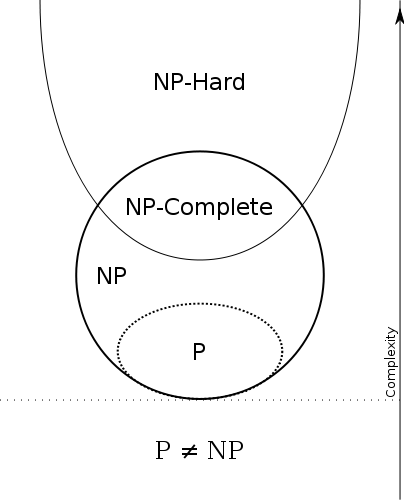
\includegraphics[scale=0.5]{images/complexity_classes.png}
	\caption{P κλάση και NP κλάση \\ πηγή: https://jcaip.github.io/Reduction-and-Intractibility/}
\end{matlab}

Το εντυπωσιακό στην περίπτωση των NP προβλημάτων είναι ότι πολλές φορές μπορεί να μοιάζουν εντυπωσιακά πολύ με κάποιο πρόβλημα που ανήκει στην κλάση P. Για παράδειγμα, δεδομένου ενός γράφου \(G = (V,E)\), η εύρεση ενός κύκλου Euler, δηλαδή ενός κύκλου που περνά από κάθε ακμή του γράφου ακριβώς μία φορά χωρίς να υπάρχει περιορισμός στο πλήθος των επισκέψεων ανά κόμβο έχει πολυπλοκότητα \(Ο(|Ε|)\). Να σημειώσουμε εδώ ότι ο παραπάνω κύκλος καλείται κύκλος Euler. Αντιθέτως, η εύρεση αν ένα γράφημα περιέχει κύκλο Hamilton, δηλαδή κύκλο που διέρχεται από κάθε κόμβο του γραφήματος ακριβώς μία φορά, είναι NP-πλήρες πρόβλημα. (Για περισσότερες πληροφορίες σχετικά με τα γραφήματα και τους κύκλους Hamilton μπορεί κανείς να ανατρέξει στην υποενότητα "Γραφήματα" της ενότητας "Μαθηματικό υπόβαθρο"). \\ 

\begin{mylemma}{TSP}{}
	Tο πρόβλημα του περιοδεύοντος πωλητή ανήκει στην κλάση NP.	
\end{mylemma}
 
Απόδειξη: \\
Για να αποδείξουμε ότι το TSP ανήκει στην κλάση NP αρκεί να βρούμε έναν αλγόριθμο, ο οποίος να επαληθεύει μία δεδομένη λύση σε πολυωνυμικό χρόνο. Έστω γράφημα \(G = (V,E)\) και \(k\) να είναι ένα threshold για την απόσταση που μπορεί να διανύσει ο πωλητής στην περίπτωση της βέλτιστης διαδρομής. Αν μία προτεινόμενη λύση είναι ένας κύκλος \(h\), τότε ο πολυωνυμικός αλγόριθμος που επαληθεύει μία λύση είναι ο παρακάτω. 

\begin{algorithm}[H]
	\SetAlgoLined
	\KwIn{Γράφημα \(G = (V,E)\), αριθμός \(k\) και κύκλος h}
	\KwResult{Απαντά ΝΑΙ στην περίπτωση που το h επαληθεύει λύση, αλλιώς απαντά ΟΧΙ}
	
	\If{h είναι Hamiltonian κύκλος του G}
	{
		sum = Υπολόγισε το άθροισμα των βαρών του h \;
		\If{sum \(\leq\) k}
		{
			Τύπωσε ΝΑΙ \;
		}
		\Else
		{
			Τύπωσε ΟΧΙ \;}
		}
	\Else
	{
		Τύπωσε ΟΧΙ \;
	}
	
	\caption{Επαλήθευση λύσης}
\end{algorithm}

Συνεπώς, το TSP είναι πρόβλημα που ανήκει στην κλάση NP. \\

Ένα σύνολο των προβλημάτων που ανήκουν στην κλάση NP καλούνται NP-complete και συγκροτούν ένα σύνολο προβλήματων NP. Πιο συγκεκριμένα, ένα πρόβλημα καλείται NP-complete αν ανήκει στην κλάση NP και κάθε άλλο πρόβλημα που ανήκει στην κλάση NP ανάγεται σε αυτό. Στο σημείο αυτό θα αποδείξουμε ότι το TSP είναι NP-complete. \\

\begin{mylemma}{TSP}{}
	Tο πρόβλημα του περιοδεύοντος πωλητή είναι NP-complete.	
\end{mylemma}

Απόδειξη: \\
Για να αποδείξουμε ότι το TSP είναι NP-complete πρέπει να αποδείξουμε ότι ανήκει στην κλάση NP και έπειτα να κάνουμε αναγωγή από ένα ήδη γνωστό NP-complete πρόβλημα. \\
Το πρώτο βήμα είναι εύκολο. Όπως αποδείχθηκε στο Λήμμα 4.0.1 το TSP ανήκει στην κλάση NP. \\
Για το δεύτερο βήμα επικαλούμαστε το πρόβλημα ύπαρξης κύκλου Hamilton σε ένα γράφημα, το οποίο είναι NP-complete. Θα ανάγουμε το πρόβλημα αυτό στο πρόβλημα του περιοδεύοντος πωλητή. \\
Έστω ότι έχουμε ένα στιγμιότυπο του προβλήματος εύρεσης κύκλου Hamilton και το γράφημα \(G = (V,E)\). Θα κατασκευάσουμε ένα καινούριο γράφημα \(G' = (V',E')\) όπου \(V' = V\) και \(E'\) θα περιλαμβάνει όλες τις δυνατές ακμές στο γράφημα. Κάθε ακμή στο \(G'\) θα έχει βάρος 1 αν είναι ακμή που υπήρχε και στο \(G\), αλλιώς θα έχει βάρος 2. Η κατασκευή ενός γραφήματος \(G'\) γίνεται σαρώνοντας το \(G\) και προσθέτοντας τις ακμές που λείπουν με κατάλληλα βάρη. Συνεπώς, η διαδικασία αυτή έχει πολυωνυμική πολυπλοκότητα. \\
Ως threshold της απόστασης του μονοπατιού που θα διανύσει ο πωλητής θέτουμε το \(|V|\). \\
Αν το \(G\) έχει Hamiltonian κύκλο, τότε και το \(G'\) θα έχει, αφού αποτελείται από τις ίδιες κορυφές και \(Ε \subseteq E'\). Ο κύκλος θα έχει άθροισμα βαρών ακμών ίσο με \(|V|\).
Αν το \(G'\) έχει Hamilton κύκλο με άθροισμα βαρών ακμών ίσο με \(|V|\), τότε ο κύκλος αυτός απαρτίζεται μόνο από τις κορυφές που έχουν βάρος 1, δηλαδή τις κορυφές που υπάρχουν και στο γράφημα \(G\). Συνεπώς, και το \(G\) έχει κύκλο Hamilton. \\
Συνεπώς, το TSP είναι NP-complete, γιατί είναι τόσο δύσκολο όσο το πρόβλημα ύπαρξης Hamilton κύκλου. \\

Στο σημείο αυτό κρίνεται σκόπιμο να αναφέρουμε ότι ο αποδοτικότερος τρόπος να μεταβεί κάποιος από ένα σημείο \(x\) σε ένα σημείο \(y\) είναι μεταβαίνοντας απευθείας στο \(y\) χωρίς ενδιάμεσους σταθμούς. Συνεπώς, η εξάλειψη των ενδιάμεσων σταθμών αποκλείεται να αυξήσει το κόστος της διαδρομής. Αυτό είναι μία ιδιότητα που αποτυπώνεται στην τριγωνική ανισότητα. 

\begin{align*}
	w(x,y) \leq w(x,z) + w(z,y)
\end{align*}

όπου \(w(x,y)\) το κόστος μετάβασης από το σημείο \(x\) στο σημείο \(y\). \\

Αν οι πόλεις που πρόκειται να επισκεφτεί ο πλανόδιος πωλητής είναι σημεία στο επίπεδο και η απόσταση μετράται με την Ευκλείδια απόσταση, τότε η τριγωνική ανισότητα ικανοποιείται και υπό αυτές τις συνθήκες το TSP είναι NP-complete, με άλλα λόγια δεν περιμένουμε αλγόριθμο που να επιλύει το πρόβλημα σε πολυωνυμικό χρόνο , αλλά κάποιον προσεγγιστικό αλγόριθμο. \\

Ένας προσεγγιστικός αλγόριθμος υπολογίζει σχεδόν βέλτιστες λύσεις και συνήθως αυτές αρκούν για τα NP-complete προβλήματα. Ένας προσεγγιστικός αλγόριθμος επιτυγχάνει λόγο προσέγγισης \(ρ(n)\), όπου \(n\) το μέγεθος της εισόδου του αλγορίθμου. Για τον \(ρ(n))\) ισχύει ότι

\begin{align*}
	\max\left(\frac{C}{C_{OPT}}, \frac{C_{OPT}}{C}\right) \leq ρ(n)
\end{align*}  

όπου \(C\) και \(C_{OPT}\) το κόστος της λύσης του προσεγγιστικού αλγορίθμου και της βέλτιστης λύσης αντίστοιχα. Ένας αλγόριθμος που επιτυγχάνει λόγο προσέγγισης \(ρ(n)\) καλείται \(ρ(n)\)-προσεγγιστικός. \\

\chapter{Μαθηματικό υπόβαθρο}

Η μελέτη σε βάθος του προβλήματος του περιοδεύοντος πωλητή χρήζει απαραίτητη την γνώση μερικών βασικών μαθηματικών εννοιών. Στο κεφάλαιο αυτό, παρουσιάζουμε και αναλύυμε, στον βαθμό που κρίνεται απαραίτητο, όλες τις μαθηματικές γνώσεις που χρειάζονται για την κατανοήση του TSP. \\

\section{Γραφήματα}

Βασική έννοια για τη μελέτη του προβήματος του περιοδέυοντος πωλητή είναι τα γραφήματα. Τα γραφήματα είναι ένα πολύ σημαντικά εργαλείο στα χερια των θεωρητικών πληροφορικών. Προσφέρουν πολλές διευκολύνσεις κατά τη μελέτη προβλημάτων (όπως και στην περίπτωση μας), είναι σχετικά απλά στη μελέτη και την κατανόηση τους και μπορούν εύκολα να κωδικοποιηθούν και να θεμελιωθούν με αυστηρό, μαθηματικό τρόπο. \\

\subsection{Βασική ορολογία}

Τα βασικά συστατικά ενός γραφήματος είναι  οι κορυφές και οι ακμές. Οι κορυφές ενώνονται με τη βοήθεια των ακμών και δημιουργούν ένα γράφημα. \\

Τα γραφήματα μπορούν να διακριθούν σε δύο βασικές κατηγορίες, τα κατευθυνόμενα γραφήματα και τη μη κατευθυνόμενα. \\

Ο αφηρημένος ορισμός στην περίπτωση των κατευθυνόμενων γραφημάτων περιλαμβάνει ένα διατεταγμένο ζεύγος \((V,E)\), όπου \(V\) είναι το σύνολο και το \(E\) είναι μία διμελής σχέση. Το \(V\) αποτελεί το σύνολο των κορυφών και το \(E\) το σύνολο των ακμών. Το κατευθυνόμενο γράφημα συμβολίζεται με \(G\). Ένα κατευθυνόμενο γράφημα μπορεί να αναπαρασταθεί γεωμετρικά ως ένα σύνολο από \(V\) σημεία, τα οποία ενώνονται με \(E\) βέλη. Ενα παραδειγμα γράφου φαίνεται στην εικόνα παρακάτω.

\begin{matlab}
	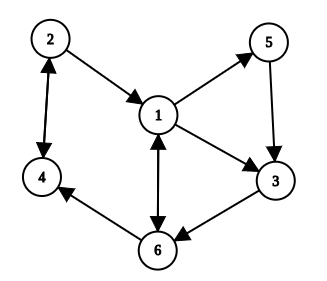
\includegraphics[scale=0.8]{images/directed_graph_example.png}
	\caption{Παράδειγμα κατευθυνόμενου γράφου \\ κατασκευάστηκε με: https://csacademy.com/app/graph\_editor/}
\end{matlab} 

Ο ορισμός για το μη κατευθυνόμενο γράφημα περιλαμβάνει ένα σύνολο \(V\) και ένα σύνολο πολυσυνόλων δύο στοιχείων \(E\). Το \(V\) αποτελεί και σε αυτήν την περιπτωση το σύνολο των κορυφών και το \(E\) το σύνολο των ακμών. Μία ενδεικτική γεμετρική αναπαράσταση δίνεται στην αντίστοιχη εικόνα παρακάτω. Και σε αυτήν την περίπτωση το \(V\) είναι ένα σύνολο σημείων, ωστόσο το \(E\) είναι ένα σύνολο γραμμών που δεν υποδικνύουν καμμία κατεύθυνση. \\

\begin{matlab}
	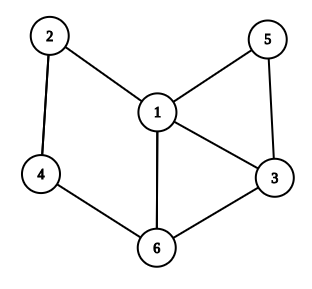
\includegraphics[scale=0.8]{images/undirected_graph_example.png}
	\caption{Παράδειγμα μη κατευθυνόμενου γράφου \\ κατασκευάστηκε με: https://csacademy.com/app/graph\_editor/}
\end{matlab}   

\subsection{Μονοπάτια}

Σε κάθε κατευθυνόμενο γράφημα οι ακμές περιέχουν μία αρχική κορυφή και μία τερματική κορυφή. Για παράδειγμα η ακμή (1,3) της εικόνας 3.1 περιέχει δύο κορυφές. Η κορυφή 1 καλείται αρχική κορυφή και η κορυφή 3 καλείται τερματική κορυφή. \\

Στα κατευθυνόμενα γραφήματα, μία ακολουθία ακμών \((e_1, e_2,...,e_k)\) όπου η τερματική κορυφή μίας ακμής \(e_j\) ταυτίζεται με την αρχική κορυφή της \(e_{(j+1)}\) καλείται μονοπάτι. \\

Αν ένα μονοπάτι δεν περιέχει την ίδια ακμή δύο φορές ονομάζεται απλό μονοπάτι. \\

Στοιχειώδες μονοποάτι καλείται το μονοπάτι εκείνο όπου δεν περιέχει την ίδια κορυφή παραπάνω από μία φορά. \\

Κύκλωμα καλείται το μονοπάτι \((e_1, e_2,...,e_k)\), όπου η τερματική κορυφή της \(e_k\) ακμής συμπίπτει με την αρχική κορυφή της \(e_1\) ακμής. \\

\subsection{Χαμιλτόνειοι κύκλοι και μονοπατια}

O Ιρλανδός φυσικός και μαθηματικός William Rowan Hamilton (4 Αυγούστου 1805 – 2 Σεπτεμβρίου 1865) μελέτησε εκτός των άλλων και τα γραφήματα. Συγκεκριμένα, δημιούργησε το μαθηματικό παιχνίδι "ο γύρος του κόσμου", του οποίου σκοπός ήταν η εύρεση ενός μονοπατιού από ακμές δωδεκαέδρου. Το μονοπάτι έπρεπε να περνά από κάθε κορυφή του δωδεκαέδρου ακριβώς μία φορά. Πιο συγκεκριμένα, ο ένας παίκτης κάρφωνε από μία βελόνα σε 5 διαδοχικές κορυφές και έπειτα ο άλλος παίκτης έπρεπε να συμπληρώσει το κύκλωμα έτσι ώστε να περιλαμβάνει όλες τις κορυφές. Μάλιστα, σε επιστολή προς τον φίλο του John T. Graves (17 Οκτωβρίου 1856) ο Hamilton τον πληροφορεί σχετικά με ένα παιχνίδι που βασίζεται στον εικοσιανό λογισμό (αλγεβρική δομή για τον υπολογισμών συμμετριών του εικοσαέδρου από τον ίδιο τον Hamilton) και την αναγνωρισιμότητα που έχει λάβει από μερικούς νεαρούς. Το παιχνίδι αυτό στάθηκε η αφορμή για την ανάπτυξη της θεωρίας γύρω από τα γραφήματα και προς τιμήν του Hamilton και του εν λόγω παιχνιδιού που επινόησε οι Χαμιλτονειανοί κύκλοι έλαβαν το όνομά του. \\

\begin{matlab}
	\includegraphics[scale=0.2]{images/Hamilton.png}
	\caption{William Rowan Hamilton \\ πηγή: https://en.wikipedia.org/wiki/William\_Rowan\_Hamilton}
\end{matlab}  

Η εύρεση ενός μονοπατιού ή ενός κυκλώματος που περνά από κάθε κορυφή ενός δεδομένου γραφήματος μόνο μία φορά φαντάζει αρχικά απλή υπόθεση, ωστόσο οι μέχρις στιγμής επιστημονικές προσεγγίσεις αποδεκνύουν το αντίθετο. 

Μονοπάτι (ή κύκλωμα) Hamilton είναι ένα μονοπάτι (ή ένα κύκλωμα) που περνά από όλες τις κορυφές ενός γραφήματος ακριβώς μία φορά. \\

Ένα γράφημα που περιέχει κύκλο Hamilton καλείται χαμιλτόνειο, ενώ αν δεν περιέχει καλείται μη χαμιλτόνειο. \\

Δυστυχώς, μέχρι και τώρα δε γνωρίζουμε κάποια ικανή και αναγκάια συνθήκη για την ύπαρξη μονοπατιών και κυκλωμάτων Hamilton. Δοθέντος ενός γραφήματος G, η απόδειξη ύπαρξης ή μη ενός μονοπατιού ή κυκλώματος Hamilton είναι η κατασκευή του. \\ 

\section{Delaunay Τριγωνοποίηση}

Στη υπολογιστική γεωμετρία, η τριγωνοποίηση πολυγώνων είναι ένα βασικό ζήτημα μελέτης. Με το όρο τριγωνοποίηση εννοούμε την διαμέριση της περιοχής που ορίζεται από το πολύγωνο σε τρίγωνα των οποίων η ένωση παράγει την περιοχή του αρχικού πολυγώνου. \\

Ουσιαστικά, η τριγωνοποίηση ενός συνόλου σημείων στο επίπεδο είναι ένα σύνολο τριγώνων. Η ένωση των τριγώνων αυτών ισούται με το κυρτό περίβλημα των σημείων και η τομή δύο τριγώνων μπορεί να είναι είτε κενή, είτε να είναι ίση με την κοινή κορυφή των δύο τριγώνων ή με την κοινή τους ακμή.

\begin{matlab}
	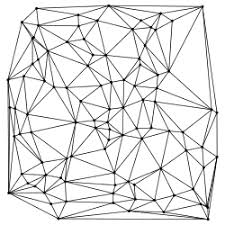
\includegraphics[scale=0.9]{images/delaunay_trianglulation.jpeg}
	\caption{Τριγωνοποίηση Delaunay \\ πηγή: https://en.wikipedia.org/wiki/Delaunay\_triangulation}
\end{matlab}

Στην παρούσα υποενότητα θα αναφερθούμε στη Delaunay τριγωνοποίηση, καθώς θα μας φανεί χρήσιμη στη μελέτη του προβλήματος του περιοδεύοντος πωλητή, με τρόπο που περιγράφεται σε επόμενη ενότητα. Επισημαίνουμε τη βασική θεωρία γύρω από την εν λόγω τριγωνοποίηση και μερικούς θεμελιώδεις αλγορίθμους που την παράγουν. \\

\subsection{Ιστορία}

Η delaunay τριγωνοποίηση ήταν μία επινόηση του Ρώσου μαθηματικού Boris Nikolaevich Delone. Ο Delone γεννήθηκε στις 15 Μαρτίου του 1890 και πέθανε έπειτα από 90 χρόνια, στις 17 Ιουλίου του 1980. Ο Boris Delone ασχολήθηκε με την άλγεβρα και τη γεωμετρία και μία από τις σημαντικότερες ανακαλύψεις του ήταν η τριγωνοποίηση Delaunay το 1934. \\

Η τριγωνοποίηση έλαβε το όνομα Delaunay, προς τιμήν του δημιουργού της, ο οποίος καλούσε τον εαυτό του "Boris Nikolaeviq Delone". Καθώς την εποχή εκείνη οι δύο επικρατέστερες γλώσσες στους επιστημονικούς κόλπους ήταν τα γαλλικά και τα γερμανικά, επικράτησε η γαλλική εκδοχή του ονόματός του και έτσι η τριγωνοποίηση έλαβε τελικά το όνομα Delaunay. \\

\begin{matlab}
	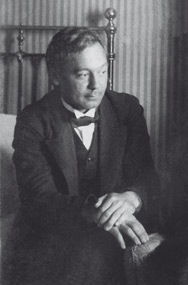
\includegraphics[scale=0.9]{images/Delone.jpg}
	\caption{Boris Nikolaevich Delone \\ πηγή: https://en.wikipedia.org/wiki/File:Delone\_cropped\_1924.jpg}
\end{matlab} 

\subsection{Βασική θεωρία}

Στόχος της τριγωνοποίησης Delaunay είναι με βάση ένα σύνολο σημείων στο επίπεδο να παράξει μία τριγωνοποίηση αυτών, η οποία να ικανοποιεί ορισμένες συνθήκες. \\

Για να μελετήσουμε την τριγωνοποίηση Delaunay πρέπει εξ αρχής να κάνουμε την παραδοχή ότι τα σημεία που πρόκειται να τριγωνοποιηθούν βρίσκονται σε γενική θέση. Γενική θέση στην παρούσα ενότητα εννοούμε ότι τέσσερα σημεία δε βρίσκονται πάνω στον ίδιο κύκλο.   \\

Αρχικά, εισάγουμε την απαραίτητη έννοια του "διανύσματος γωνιών" (vector angle). Έστω ότι \(P := \left\{ p_1, p_2,...,p_n \right\}\) είνα ένα σύνολο \(n\) σημείων στο επίπεδο. Επίσης, έστω ότι \(Τ\) είναι μια τριγωνοποίησή τους. Αν \(m\) είναι το σύνολο των τριγώνων που έχουν παραχθεί στη συγκεκριμένη τριγωνοποίηση, τότε με προφανή τρόπο εξάγεται το συμπέρασμα ότι το σύνολο των γωνιών που περιέχει η τριγωνοποίηση είναι \(3m\). Τοποθετούμε τις γωνίες της τριγωνοποίησης σε ένα διάνυσμα σε αύξουσα σειρά. Το διάνυσμα αυτό καλείται vector-angle και ορίζεται ως εξής

\begin{align}
	A(T) := (a_1, a_2, ..., a_{3m})
\end{align}   

όπου

\begin{align}
	a_i \leq a_j \text{, } \forall i<j
\end{align}

Αν \(Τ'\) είναι μια διαφορετική τριγωνοποίηση από την \(Τ\) για το ίδιο σύνολο σημείων \(P\) και το αντίστοιχο διάνυσμα γωνιών είναι το \(A(T') = (a_{1}', a_{2}', ..., a_{3m}')\), θα λέμε ότι το διάνυσμα γωνιών της \(Τ\) τριγωνοποίησης είναι μεγαλύτερο από το διάνυσμα γωνιών της \(Τ'\) τριγωνοποίησης και θα γράφουμε \(Α(Τ) > Α(Τ')\) αν υπάρχει \(i\), όπου \(1 \leq i \leq 3m\) τέτοιο ώστε 

\begin{align*}
	a_j = a_{j}' \text{, } \forall j < i \text{ και } a_i > a_{i}'
\end{align*}

Θα δούμε στη συνέχεια ότι στόχος μας εδώ είναι να καταφέρουμε να εντοπίσουμε το μεγαλύτερο διάνυσμα γωνιών. \\

Θα λέμε ότι μία τριγωνοποίηση είναι "angle-optimal" και θα γράφουμε \(Α(Τ) \geq A(T')\) αν \(Α(Τ) > Α(Τ')\) για όλες τις δυνατές τριγωνοποιήσεις \(T'\). \\

Στο σημείο αυτό πρέπει να αναφέρουμε ότι το πλήθος των τριγώνων που προκύπτουν από μία τριγωνοποίηση δεν είναι τυχαίο. Μπορεί να καθοριστεί με ακρίβεια, πράγμα που ήδη έχει διατυπωθεί σε αντίστοιχο θεώρημα. \\

\begin{mytheorem}{Πλήθος ακμών και τριγώνων τριγωνοποίησης σημείων στο επίπεδο}{Α}
	Έστω \(P\) ένα σύνολο \(n\) σημείων στο επίπεδο. Έστω ότι τα σημεία δεν είναι όλα μεταξύ τους συνευθειακά και έστω με \(k\) να συμβολίζονται ότα τα σημεία που βρίσκονται στο όριο του convex hull του \(P\). Οποιαδήποτε τριγωνοποίηση των σημείων του \(P\) παράγει \(2n - 2 - k \) τρίγωνα και \(3n - 3 - k\) ακμές.
\end{mytheorem}

Απόδειξη: \\
Έστω ότι τα \(P\) σημεία τριγωνοποιούνται και παράγονται \(m\) το πλήθος τρίγωνα. Συνεπώς, το επίπεδο έχει διαχωριστεί με \(m + 1\) υποπεριοχές. \\
Κάθε τρίγωνο έχει 3 ακμές και το convex hull έχει \(k\) ακμές. \\
Κάθε ακμή ανήκει σε δύο υποπεριοχές του επιπέδου. \\
Συνεπώς, ο συνολικός αριθμός ακμών είναι  \(\frac{3m + k}{2}\). \\
Από τον τύπο του Euler, όπου \(n_f = m + 1\) και \(n_e = \frac{3m + k}{2}\), προκύπτει ότι 

\begin{align*}
	n - n_e + n_f= 2 & \Leftrightarrow \\
	n - \frac{3m + k}{2} + (m+1) = 2 & \Leftrightarrow \\	
	2n - (3m + k) + 2(m+1) = 4 & \Leftrightarrow \\
	2n - 3m - k + 2m + 2 = 4 & \Leftrightarrow \\
	2n - m - k = 2 & \Leftrightarrow \\
	m = 2n - k - 2
\end{align*}

και αφού \(m = 2n - 2 - k\), το \(n_e\) υπολογίζεται να είναι

\begin{align*}
	n_e = \frac{3m + k}{2} & \Leftrightarrow \\
	n_e = \frac{3(2n - k - 2) + k}{2} & \Leftrightarrow \\
	n_e = \frac{6n - 3k - 6 + k}{2} & \Leftrightarrow \\
	n_e = \frac{6n - 6 - 2k}{2} & \Leftrightarrow \\
	n_e = 3n - 3 - k
\end{align*}

\(\square \)

Όπως ήδη αναφέραμε στόχος είναι να βρεθεί η τριγωνοποίηση που δίνει το "μεγαλύτερο" διάνυσμα γωνιών. Για να καταφέρουμε να φτάσουμε στο σημείο να παράξουμε μία τέτοια τριγωνοποίηση για ένα δεδομένο σύνολο σημείων πρέπει να αναφέρουμε μερικές ακόμα θεμελιώδεις έννοιες. Εισάγουμε την έννοια της "παράνομης ακμής" (illegal edge). \\

Έστω μία τριγωνοποίηση των \(P\) σημείων και έστω μία ακμή της τριγωνοποίησης που βρίσκεται εντός ενός κυρτού τετράπλευρου και είναι κοινή ακμή για δύο διαφορετικά τρίγωνα της τριγωνοποίησης. Η ακμή αυτή μπορέι να γίνει flip. Στην περίπτωση αυτή το μόνο που αλλάζει είναι το \(A(T)\). \\

\begin{mydefinition}{Παράνομη ακμή}{α}
	Έστω \(T\) μία τριγωνοποίηση των σημείων \(P\).  Καλούμε μία ακμή "παράνομη" εαν μπορούμε να αυξήσουμε τη μικρότερη γωνία του διανύσματος γωνιών κάνοντάς την flip.
\end{mydefinition}

Αν \(T\) μία τριγωνοποίηση που περιέχει μία παράνομη ακμή και \(T'\) η τριγωνοποίηση που έχει γίνει flip η παράνομη ακμή, τότε ισχύει ότι η \(T'\) είναι angle-optimal:

\begin{align*}
	A(T') \geq A(T)
\end{align*}

\begin{mydefinition}{}{}
	Μία τριγωνοποίηση \(T\) καλείται νόμιμη εαν δεν περιέχει καμία παράνομη ακμή.
\end{mydefinition}

Συνεπώς, κάθε angle-optimal τριγωνοποίηση είναι νόμιμη. \\

Με βάση αυτήν την τεχνική μπορούμε να οδηγηθούμε σε μία τριγωνοποίηση Delaunay. \\

\begin{mydefinition}{Τριγωνοποίηση Delaunay}{}
	Για ένα σύνολο σημείων \(P\) στο επίπεδο, η τριγωνοποίηση Delaunay είναι η τριγωνοποίηση εκείνη που δεν περιέχει καμία παράνομη ακμή. Συμβολίζουμε την τριγωνοποίηση Delaunay των σημείων με \(Del(P)\).
\end{mydefinition}

Μία εναλλακτική προσέγγιση των flips και των ελέγχων των διανυσμάτων γωνιών για την παραγωγή Delaunay τριγωνοποίησης είναι η προσέγγιση με τη βασικό εργαλείο τον κύκλο. Στο σημείο αυτό, επισημαίνουμε κάποιες βασικές ιδιότητες που αφορούν τον κύκλο και πηγάζουν από το θεώρημα του Θαλή. \\

\begin{matlab}
	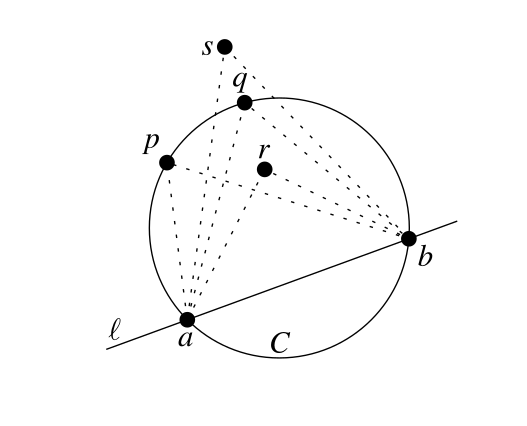
\includegraphics[scale=0.4]{images/circle.png}
	\caption{Κύκλος C με τόξο ab \\ πηγή: "Computational Geometry, Algorithms and Applications,Third Edition", σελ. 194}
\end{matlab}

\begin{mytheorem}{Γωνίες που βαίνουν σε χορδή}{χορδη1}
	Έστω \(C\) να είναι ένας κύκλος και \(l\) μία ευθεία που τέμνει τον κύκλο στα σημεία \(a\) και \(b\). Έστω \(p\) και \(q\) σημεία πάνω στην περίμετρο του κύκλου. Τότε η γωνία που βαίνει στο τόξο \(ab\) με κορυφή το σημείο \(p\) είναι ίση με την γωνία που βαίνει στο ίδιο τόξο και έχει κορυφή το σημείο \(q\). 
\end{mytheorem}

\begin{mytheorem}{Γωνίες που βαίνουν σε χορδή}{χορδη2}
	Έστω \(C\) να είναι ένας κύκλος και \(l\) μία ευθεία που τέμνει τον κύκλο στα σημεία \(a\) και \(b\). Έστω \(r\) ένα σημείο εντός του κύκλου και \(s\) ένα σημείο εκτός. Τότε η γωνία που βαίνει στο τόξο \(ab\) με κορυφή το σημείο \(r\) είναι μεγαλύτερη από την γωνία που βαίνει στο ίδιο τόξο και έχει κορυφή το σημείο \(s\). 
\end{mytheorem}

Συνοψίζοντας 

\begin{align}
	\angle arb > \angle apb = \angle aqb > \angle asb
\end{align}

Από όλα τα παραπάνω προκύπτει ότι \\

\begin{mylemma}{}{}
	Έστω \(C\) ένας κύκλος και \(p_i, p_j, p_k\) σημεία πάνω στον κύκλο και \(p_l\) σημείο εντός του κύκλου. Αν τα \(p_i, p_j, p_k, p_l\) σχηματίζουν ένα κυρτό πολύγωνο, τότε αυτό μπορεί να τριγωνοποιηθεί και να παραχθούν τα τρίγωνα \(p_i p_j p_k\) και \(p_i p_j p_l\) με κοινή ακμή την \(p_i p_j\). Η ακμή \(p_i p_j\) είναι παράνομη.
\end{mylemma} 

\begin{mylemma}{}{}
	Έστω \(C\) ένας κύκλος και \(p_i, p_j, p_k\) σημεία πάνω στον κύκλο και \(p_l\) σημείο εκτός του κύκλου. Αν τα \(p_i, p_j, p_k, p_l\) σχηματίζουν ένα κυρτό πολύγωνο, τότε αυτό μπορεί να τριγωνοποιηθεί και να παραχθούν τα τρίγωνα \(p_i p_j p_k\) και \(p_i p_j p_l\) με κοινή ακμή την \(p_i p_j\). Η ακμή \(p_i p_j\) είναι νόμιμη.
\end{mylemma} 

Φυσικά, να υπενθυμίσουμε ότι τα σημεία βρίσκονται σε γενική θέση, συνεπώς δεν παίρνουμε την περίπτωση τα \(p_i, p_j, p_k, p_l\) να είναι και τα 4 πάνω στον ίδιο κύκλο. \\

Στο παραακάτω θεώρημα συνοψίζεται η προσέγγιση της τριγωνοποίησης με εργαλείο τον κύκλο. \\

\begin{mytheorem}{Η ιδιότητα των κενών κυκλων}{}
	Έστω \(P\) ένα σύνολο σημείων στο επίπεδο που βρίσκονται σε γενική θέση. Μία τριγωνοποίηση \(T\) είναι τριγωνοποίηση Delaunay αν και μόνο αν ο κυκλος που σχηματίζεται από κάθε τριάδα σημείων που αποτελούν τρίγωνο της τριγωνοποίησης δεν περιέχει κανένα άλλο σημείο του \(P\) στο εσωτερικό του.
\end{mytheorem} 

Απόδειξη: \\
\(\Rightarrow \) \\
Αν κανένα σημείο του συνόλου σημείων \(P\) δεν βρίσκεται εσωτερικά του εκάστοτε κύκλου που σχηματίζεται από τις τρεις κορυφές ενός τριγώνου της τριγωνοποίησης, τότε όλες οι ακμές είναι νόμιμες. Συνεπώς, η τριγωνοποίηση είναι νόμιμη. \\
\(\Leftarrow \) "Αν μια τριγωνοποίηση είναι Delaunay, τότε κανένα σημείο του \(P\) δεν βρίσκεται εντός του εκάστοτε κύκλου τριών κορυφών τριγώνου της τιγωνοποίησης" \\
Θα αποδείξουμε αυτήν την κατεύθυνση με απαγωγή σε άτοπο. \\
Έστω ότι η τριγωνοποίηση \(T\) είναι τριγωνοποίηση Delaunay και έστω ότι υπάρχει κύκλος που περιέχει σημεία του \(P\) εκτός των \(A, B, C\) που τον ορίζουν και είναι οι κορυφές ενός τριγώνου της τριγωνοποίησης. \\
Έστω ότι από όλα αυτά τα σημεία επιλέγεται εκείνο που απέχει την μικότερη απόσταση απο την ακμή του τριγώνου, έστω \(D\). \\
Επειδή η τριγωνοποίηση είναι Delaunay, το τρίγωνο \(BCD\) δε μπορεί να ανήκει στην τριγωνοποίηση. \\
Έστω \(Ε\) ένα σημείο εκτός του κύκλου και \(BCE\) τρίγωνο. Το \(D\) βρίσκεται εντός του κύκλου που ορίζεται από τα σημεία \(B, C, E\) και εκτός του τριγώνου \(BCE\). 
......................................

\begin{matlab}
	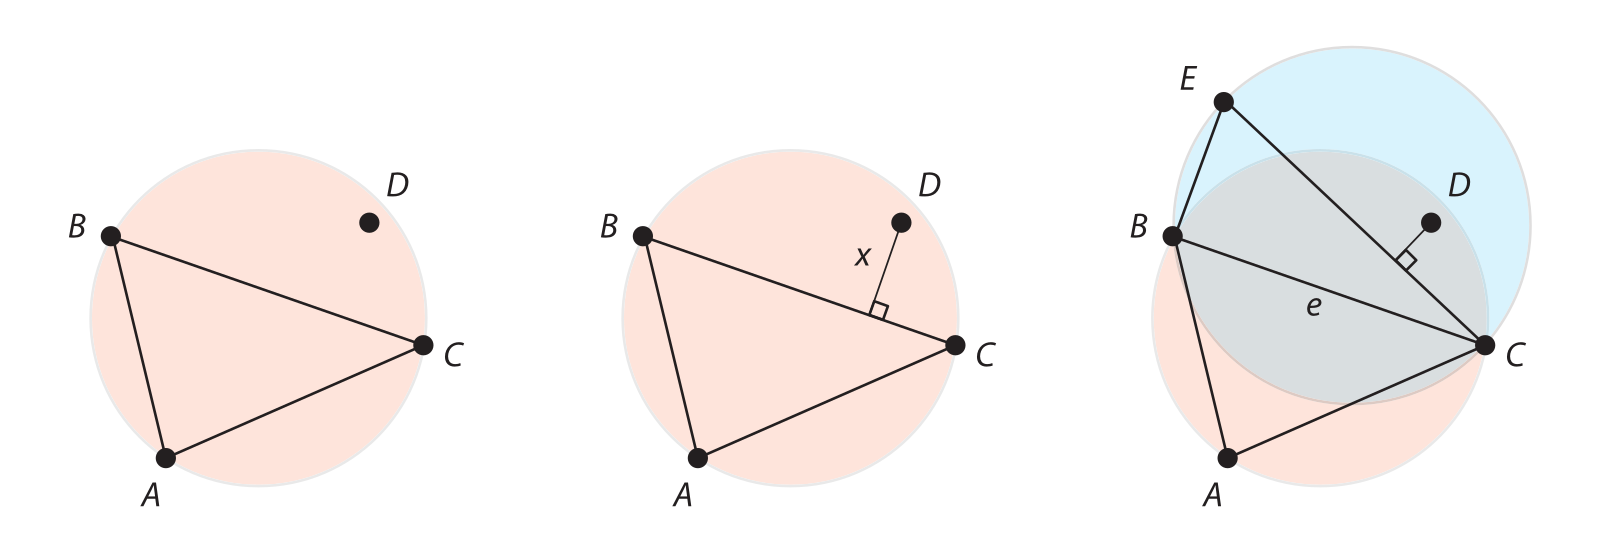
\includegraphics[scale=0.3]{images/emptycircle.png}
	\caption{Απόδειξη του θεωρήματος 3.2.4 \\ πηγή: "Discrete and Computational Geometry", σελ.: 86}
\end{matlab} 

Συνοψίζουμε τα κριτήρια για την Delaunay τριγωνοποίηση σε ένα θεώρημα. \\

\begin{mytheorem}{Delaunay Τριγωνοποίηση}{}
	Σε μία τριγωνοποίηση Delaunay \(T\) των σημείων \(P\): \\
	1. Τρία σημεία κατασκευάζουν τρίγωνο αν και μόνο αν ο περιγεγραμμένος ανοιχτός κύκλος του δεν περιέχει κανένα άλλο σημείο του \(P\). \\
	2. Δύο σημεία κατασκευάζουν ακμή αν και μόνο αν υπάρχει κύκλος με τα σημεία αυτά στην περιφέρειά του που δεν περιέχει κανένα άλλο σημείο του \(P\) 	
\end{mytheorem}

Για δεδομένη τριγωνοποίηση, θα αποφασίζουμε αν αυτή είναι Delaunay ανν ο περιγεγραμμένος κύκλος κάθε τριγώνου δεν περιέχει κανένα άλλο σημείο. \\

\subsection{Κατασκευή Delaunay Τριγωνοποίησης}

Αφού είδαμε τη θεωρητική βάση της τριγωνοποίησης Delaunay, μπορούμε πλέον να αναφερθούμε σε τεχνικές και αλγόριθμους που κατασκευάζουν μία τριγωνοποίηση Delaunay. \\

\subsubsection{Αυξητκός αλγόριθμος}

Ο αλγόριθμος αυτός δε γνωρίζει εκ των προτέρων όλα τα σημεία που πρόκειται να τριγωνοποιηθούν. Για τη ακρίβεια, λαμβάνει ένα σύνολο σημείων, σε κάθε βήμα του εξετάζει ενα απο τα σημεία αυτά και παράγει την τρέχουσα Delaunay τριγωνοποίηση σαν να μην υπάρχουν άλλα σημεία προς εξέταση, μέχρι που εξετάζει όλο το σύνολο σημείων και παράγει της τελική Delaunay τριγωνοποίηση. Η επιλογή σημείου σε κάθε βήμα γίνεται με τυχαίο τρόπο. \\

Ο αλγόριθμος έχει \(Ο(n logn)\) μέση πολυπλοκότητα, ενώ στη χείριστη περίπτωση η πολυπλοκότητά του είναι \(O(n^2)\). \\

Ο αλγόριθμος επιλέγει 3 σημεία στο επίπεδο των οποίων το αντίστοιχο τρίγωνο περιλαμβάνει όλα τα σημεία προς τριγωνοποίηση. Η επιλογή των τριών αυτών σημείων δεν είναι τυχαία και πρέπει να πληρεί ορισμένα κριτήρια. Θα αναφερθούμε σε αυτά στη συνέχεια, αφού πρώτα παρουσιάσουμε τον πυρήνα του αλγορίθμου. \\

Ο αλγόριθμος αυξητικά παράξει σε κάθε του βήμα την τριγωνοποίηση. Για κάθε σημείο που ελέγχει εντόπίζει αν βρίσκεται εντός τριγώνου της ήδη κατασκευασμένης τριγωνοποίησης ή πάνω σε κάποια ακμής της τριγωνοποίησης. Στην περίπτωση που βρίσκεται μέσα σε τρίγωνο κατασκευάζονται τρείς νέες ακμές, οι οποίες εκτείνονται από το υπό εξέταση σημείο προς την κάθε κορυφή του τριγώνου που το περιέχει. Στην περίπτωση που το σημείο βρίσκεται πάνω σε ακμή της τριγωνοποίησης είναι εύκολο κανείς να συνειδητοποιήσει ότι η ακμή αυτή είναι κοινή ακμή για δύο τριγωνα. Συνεπώς, δημιουργούνται δύο νέες ακμές από το σημείο που εξετάζεται προς τη μία κορυφη του ενός και του άλλου τριγώνου που δεν ανήκουν στο ευθύγραμμο τμήμα. Για την καλύτερη κατανόηση των δύο περιπτώσεων παρέχεται η αντίστοιχη εικόνα. Αφού δημιουργηθούν οι νέες ακμές με κατάλληλο τρόπο μένει να ελέγξουμε ότι η τριγωνοποίηση που έχει παραχθεί είναι Delaunay. Η προσθήκη μιας νέας ακμής μπορεί να κάνει παράνομες τις ήδη υπάρχουσες ακμές της τριγωνοποίησης. Αυτο αντιμετωπίζεται με κατάλληλα flips κάθε φορά. Ο αλγόριθμος παρουσιάζεται συνοπτικά παρακάτω. \\

Ο αλγόριθμος σαφώς τερματίζει, καθώς το πλήθος των ακμών της τριγωνοποίησης είναι πεπερασμένο. Επίσης, ο αλγόριθμος είναι ορθός διότι εξετάζει κάθε ακμή ως προς την "νομιμότητά" της στο βήμα όπου καλεί τον αλγόριθμο "Νομιμοποίηση ακμής". Συνεπώς, ποτέ δε θα προκύψει παράνομη ακμή χωρίς να ελεγχθεί και να μετατραπεί σε νόμιμη. όπως ήδη έχουμε αναφέρει, μια τριγωνοποίηση είναι Delaunay αν είναι νόμιμη. \\

\begin{algorithm}[H]
	\SetAlgoLined
	\KwIn{n σημεία του επιπέδου}
	\KwResult{Τριγωνοποίηση Delaunay για n σημεία του επιπέδου}
	
	Δημιούργησε κατάλληλα σημεία \(p_{-1}, p_{-2}, p_{-3}\) στο επίπεδο έτσι ώστε το τρίγωνο που σχηματίζουν να περέχει τα n σημεία εισόδου. \;
	\For{ένα σημείο του επιπέδου που δεν έχει ενταχθέι στην τριγωνοποίηση}
	{Βρες σε ποιο τρίγωνο ή ακμή ανήκει \;
	\If{σημείο ανήκει σε τρίγωνο}
		{Πρόσθεσε 3 νέες ακμές προς τις κορυφές του τριγώνου \;
		Κάλεσε τον αλγόριθμο 2 για τις 3 πλευρές του τριγώνου \;}
	\Else
		{Πρόσθεσε 2 νέες ακμές προς τις κορυφές των τριγώνων που έχουν κοινή πλευρά την πλευρά που ανήκει το υπο εξέταση σημείο \;
		Κάλεσε τον αλγόριθμο 2 για τις 4 πλευρές των 2 τριγώνων \;}
	}	
	
	\caption{Αυξητικός αλγόριθμος τριγωνοποίησης Delaunay}
\end{algorithm}

\begin{algorithm}[H]
	\SetAlgoLined
	\KwIn{Τριγωνοποίηση σημείων, ακμή της τριγωνοποίησης \(p_i p_j\), σημείο \(p_r\)}
	\KwResult{Τριγωνοποίηση που είναι νόμιμη}
	
	Βρές τρίγωνο \((p_i, p_j, p_l)\) \;
	\If{\(p_i p_j\) παράνομη}
	{Διαγραφή \(p_i p_j\) \;
	Δημιουργία \(p_r p_l\) \;
	\(p_i p_l\) = νόμιμη ως προς την \(p_r\) \;
	\(p_j p_l\) = νόμιμη ως προς την \(p_r\) \;}
	
	\caption{Νομιμοποίηση ακμής}
\end{algorithm}

\begin{matlab}
	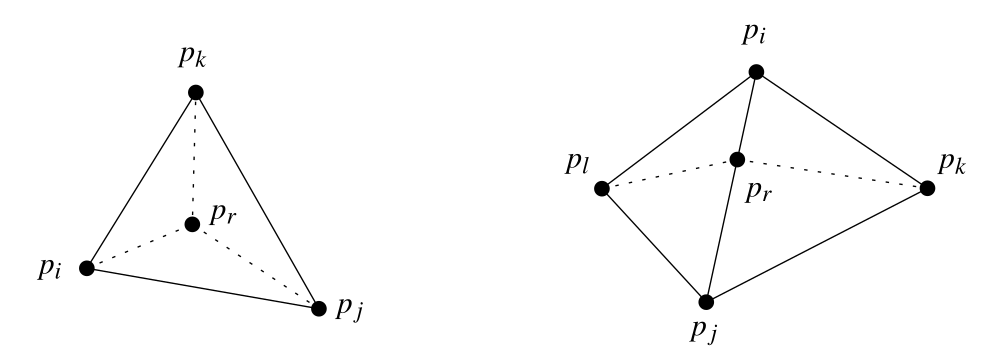
\includegraphics[scale=0.3]{images/incremental.png}
	\caption{Οι δύο περιπτώσεις που εξετάζει ο αυξητικός αλγόριθμος κατά την εισαγωγή ενός νέου σημείου \(p_r\). Αριστερά φαίνεται η πρώτη περίπτωση, όπου το νεό σημείο εντοπίζεται εντός τριγώνου της τριγωνοποίησης, ενώ δεξία φαίνεται η δεύτερη περίπτωση όπου το νέο σημείο βρίσκεται πάνω σε ακμή της τριγωνοποίησης \\ πηγή: "Computational Geometry, Algorithms and Applications, Third Edition", σελ.: 200}
\end{matlab} 

Στο σημείο αυτό μπορούμε να εξηγήσουμε τον τρόπο που επιλέγουμε τα τρία αρχικά σημεία που δημιουργούν τρίγωνο που περιβάλει όλα τα προς τριγωνοποίηση σημεία. Ουσιαστικά, τα σημεία αυτά πρέπει να λάβουν θέσεις στο επίπεδο, που να μην επηρεάζουν την έκβαση της τριγωνοποίσης μετέπειτα. Αυτό επιτυγχάνεται μόνο αν τοποθετηθούν αρκετά μακρυά από τα σημεία που πρόκειται να τριγωνοποιηθούν. Για να συμβεί αυτό πρέπει καθένα από τα σημεία \(p_{-1}, p_{-2}, p_{-3}\) να μην βρίσκονται εντός των κύκλων που σχηματίζονται από όλες τις δυνατές τριάδες σημειων. Μόνο τότε μπορούμε να είμαστε βέβαιοι ότι δεν έχουν επηρεάσει την τριγωνοποίηση Delaunay. \\

Τέλος, πρέπει να αποσαφηνίσουμε τον τρόπο με τον οποίον ο αλγόριθμος αντιλαμβάνεται πότε ένα σημείο είναι εντός τριγώνου ή πάνω σε κάποια ακμή. Αυτό επιτυγχάνεται με τη δημιουργία ενός κατάλληλου κατευθυνόμενου ακυκλικού γράφου. Ο γράφος αυτός κωδικοποιεί όλα τα τρίγωνα που δημιουγήθηκαν κατά την εκτέλεση του αλγορίθμου και την χρονική τους ιεραρχία. Οι κόμβοι είναι τρίγωνα και οι ακμές δηλώνουν τις σχέσεις μεταξύ δύο τριγώνων. Αν δύο κόμβοι συνδέονται με ακμή, δηλαδη με σχέση "πατέρα - παιδιού", τότε τα αντίστοιχα τρίγωνα έχουν μη κενή τομή. Είναι προφανές πως η ρίζα του γράφου είναι το τρίγωνο \(p_{-1} p_{-2} p_{-3}\). Έχουμε ήδη αναφέρει ότι η προσθήκη ενός νέου σημείου μπορεί να δημιουργήσει τρία ή τέσσερα τρίγωνα στην τριγωνοποίηση. Σε όρους γράφου, αυτό σημαίνει τρία ή τέσσερα νέα φύλλα. Το flip μιας ακμής δημιουργεί μόνο δύο φύλλα. \\

Για τον εντοπισμό ενός σημείου, διατρέχεται ο γράφος ξεκινόντας από τη ρίζα. Ελέγχονται τα τρία παιδία της ρίζας και εντοπίζουμε σε ποιο από αυτά τα τρία τρίγωνα (που περιέχονται στους κόμβους) ανήκει το προς εξέταση σημείο. Μεταβαίνουμε στο κατάλληλο παιδί και συνεχίζουμε την ίδια ακριβώς διαδικασία μέχρι να φτάσουμε σε φύλλο του γράφου στο οποίο και εντοπίζεται το σημείο που εξετάζουμε. \\ 

\section{Κυρτό Περίβλημα}

Πολλές φορές είναι απαραίτητο, δοθέντος ενός συνόλου σημείων (είτε στο επίπεδο, είτε σε μαγαλύτερες διαστάσεις) να βρεθεί ένα κυρτό περίβλημα που να περιέχει όλα τα σημεία στο εσωτερικό του. Εμείς θα επικεντρωθούμε στην περίπτωση όπου τα σημεία ανήκουν στο \(\R^2\). \\

Έχουμε ήδη αναφέρει μερικές έννοιες κλειδιά, ωστόσο δεν τις έχουμε ορίσει με αυστηρό τρόπο. Αρχικά, δίνουμε τον ορισμό της κυρτότητας. \\

\begin{mydefinition}{Κυρτό}{}
	Κυρτό (convex) είναι κάθε αντικείμενο ή σύνολο σημείων, στο οποίο κάθε ευθύγραμμο τμήμα με άκρα που ανήκουν στο αντικείμενο ή στο σύνολο σημείων βρίσκεται μέσα στο αντικείμενο.
\end{mydefinition}

Συνεπώς, στόχος είναι να βρεθεί μία κυρτή πολυγωνική γραμμή που να περιέχει όλα τα σημεία που επιθυμούμε. Για να συμβεί αυτό, η πολυγωνική γραμμή πρέπει να είναι κλειστή. \\

\begin{mydefinition}{Κλειστή Πολυγωνική Γραμμή}{}
	Κλειστή πολυγωνική γραμμή καλείται η πολυγωνική γραμμή της οποίας το τέλος του τελευταίου τμήματος ταυτίζεται με την αρχή του πρώτου.
\end{mydefinition}

Στο σημείο αυτό, μπορούμε να ορίσουμε το κλειστό πολύγωνο ως έννοια. \\

\begin{mydefinition}{Κλειστό Πολύγωνο}{}
	Κλειστό πολύγωνο καλείται η ένωση μιας κλειστής πολυγωνικής γραμμής και του εσωτερικού της.
\end{mydefinition}

Στο εξής, καταχρηστικά θα αναφερόμαστε στην έννοια του κλειστού πολυγώνου με τον όρο "πολύγωνο". Ο ορισμός αναφέρεται στο εσωτερικό του πολυγώνου, το οποίο μπορεί να οριστεί αυστηρά από το θεώρημα του Jordan. \\

\begin{mytheorem}{Jordan}{}
	Κάθε κλειστή και απλή επίπεδη καμπύλη χωρίζει το επίπεδο σε δύο περιοχές, το εσωτερικό και το εξωτερικό της καμπύλης.
\end{mytheorem}

Μπορούμε πλέον να ορίσουμε την έννοια του κυρτού περιβλήματος με βάση τους δύο παρακάτω ορισμούς που είναι ισοδύναμοι. \\

\begin{mydefinition}{Κυρτό Περίβλημα}{}
	Το κυρτό περίβλημα ενός συνόλου σημείων στο επίπεδο είναι το κυρτό πολύγωνο με ελάχιστο εμβαδόνπου περιλαμβάνει όλα τα δεδομένα σημεία.
\end{mydefinition}

\begin{mydefinition}{Κυρτό Περίβλημα}{}
	Το κυρτό περίβλημα (convex hull) ενός συνόλου σημείων στο επίπεδο είναι το κυρτό πολύγωνο που περιέχει τα δεδομένα σημεία και είναι ελάχιστο ως προς τη σχέση υποσυνόλου σημείων. Δεν υπάρχει κυρτό πολύγωνο που να περιέχει όλα τα δεδομένα σημεία και να είναι γνήσιο υποσύνολο του κυρτού περιβλήματος.
\end{mydefinition}

Ένα παράδειγμα convex hull δίνεται στην εικόνα. \\

\begin{matlab}
	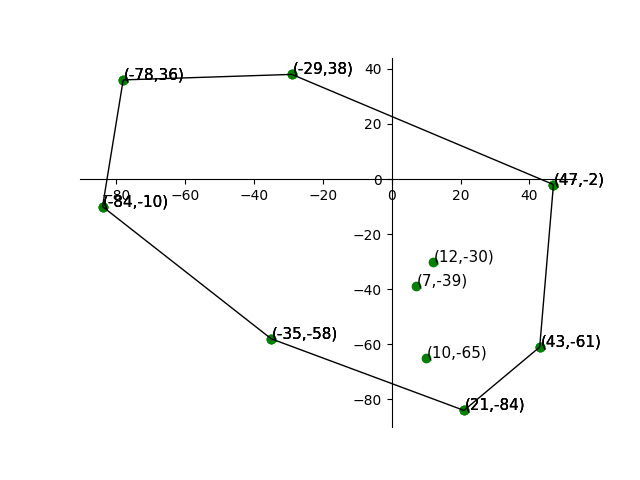
\includegraphics[scale=0.8]{images/convexhull.png}
	\caption{Παράδειγμα convex hull δέκα σημείων στο επίπεδο \\ πηγή: Output αλγορίθμου που έχουμε υλοποιήσε για την εύρεση κυρτού περιβλήματος}
\end{matlab}

Στη συνέχεια παραθέτουμε δύο βασικούς αλγορίθμους εύρεσης κυρτού περιβλήματος, τον αυξητικό αλγόριθμο και τον αλγόριθμο περιτύλιξης. Για τους δύο αλγορίθμους έχουμε υποθέσει ότι όλα τα σημεία βρίσκονται σε γενική θέση.

\begin{mydefinition}{Γενική Θέση}{}
	Ένα σύνολο σημείων στο επίπεδο βρίσκεται σε γενική θέση (generic position) για προβλήματα κυρτού περιβλήματος αν και μόνο αν οποιαδήποτε τρία σημεία δεν είναι συνευθειακα.
\end{mydefinition}

\subsection{Αυξητικός αλγόριθμος}

Ο αυξητικός αλγόριθμος ή αλλιώς beneath-beyond δημιουργεί ένα κατάλληλο κυρτό περίβλημα βασιζόμενος σε ένα σύνολο σημείων στον δισδιάστατο χώρο εν προκειμένω. Καλείται έτσι διότι εξετάζει σημεία του χώρου το ένα μετά το άλλο και κάθε φορά προσθέτει ένα σημείο στο υπό κατασκευή κυρτό περίβλημα. \\

Αρχικά, ταξινομούνται σε φθίνουσα σειρά όλα τα σημεία του δισδιάστατου χώρου με πρωτεύον κριτήριο την τετμημένη τους. Έτσι, ο αλγόριθμος ξεκινά με τα σημεία που βρίσκονται δεξιά και καταλήγει σε εκείνα που βρίσκονται αριστερά, δηλαδή σαρώνει τα σημεία από δεξιά προς αριστερά. Με αυτόν τον τρόπο κάθε καινούριο σημείο που εξετάζεται από τον αλγόριθμο είναι εξωτερικό του πολυγώνου που ήδη έχει κατασκευαστεί. Επίσης το ευθύγραμμο τμήμα που σχηματίζεται από το υπό εξέταση σημείο και από το ακριβώς προηγούμενο υπό εξέταση σημείο είναι εξωτερικό του κυρτού περιβλήματος. \\

Ξεκινώντας από τα τρία δεξιότερα σημεία δημιουργείται ένα τρίγωνο, το οποίο θεωρείται κυρτό περίβλημα στην περίπτωση που είχαμε μόνο αυτά τα τρία σημεία ως είσοδο. Ο αλγόριθμος βασίζεται στο τρίγωνο αυτό και το επεκτείνει στην κυρτή θήκη που στοχεύει να κατασκευάσει. \\

Βασικό χαρακτηριστικό του beneath-beyond είναι ο χρωματισμός των ακμών και των κορυφών. Πιο συγκεκριμένα, οι κορυφές μπορούν να λάβουν τρία διαφορετικά χρώματα και οι ακμές δύο. Μία ακμή χρωματίζεται κόκκινη στην περίπτωση που είναι ορατή από το υπό εξέταση κάθε φορά σημείο, ενώ αν δεν είναι ορατή χρωματίζεται με μπλέ χρώμα. Οι κορυφές μπορούν να λάβουν τα χρώματα: κόκκινο, μπλέ και μωβ. Μία κορυφή είναι κόκκινη όταν εντοπίζεται ανάμεσα σε δύο κόκκινες ακμές, μπλέ όταν εντοπίζεται ανάμεσα σε δύο μπλέ ακμές και μώβ όταν εντοπίζεται ανάμεσα σε μία κόκκινη και μία μπλέ ακμή. \\

Η ορατότητα κάθε ακμής από ένα σημείο υπολογίζεται με βάση το κατηγόρημα προσανατολισμού ή αλλιώς το κατηγόρημα CCW (Counter ClockWise). Ο έλεγχος αυτός μπορεί να παράξει δύο διακριτές τιμές (π.χ.: True/False). Στην περίπτωση του κατηγορήματος CCW, η είσοδός του είναι τρία σημεία και η έξοδός του είναι ο προσανατολισμός αυτών των τριών σημειών, δηλαδή η φορά της στροφής των σημείων αυτών. Αν τα τρία σημεία που δίνονται στο CCW είναι τα \(x,y,z\), το κατηγόρημα αποφασίζει αν τα διανύσματα \(\vec{v_1} = (x,y)\) και \(\vec{v_2} = (x,z)\) σύμφωνα με τον κανόνα του δεξιού χεριού ορίζουν μία θετική ή μία αρνητική στροφή. Θετική καλείται η στροφή στην οποία το εξωτερικό γινόμενο των διανυσμάτων έχει θετικό πρόσημο, ενώ σε διαφορετική περίπτωση καλείται αρνητική. Η αρνητική στροφή καλείται CW (σύμφωνη με τη φορά των δεικτών του ρολογιού) και η θετική CCW (αντίθετη με τη φορά των δεικτών του ρολογιού). Να σημειώσουμε ότι η επιλογή εδώ των διανυσμάτων έγινε με τυχαίο τρόπο και το βασικό είναι να επιλέγονται διανύσματα με κοινή κορυφή. \\

Στον αλγόριθμο η ορατότητα της ακμής καθορίζεται από τον υπολογισμό των \(CCW(a_i, a_j, a)\) και \(CCW(a_i, a_j, p)\), όπου p είναι το υπό εξεταση σημείο, τα \(a_i\) και \(a_j\) ορίζουν μία ακμή του πολυγώνου και a είναι μία οποιαδήποτε άλλη κορυφή που ανήκει στο πολύγωνο και δεν είναι μία από τις τρείς κορυφές που αναφέρθηκαν παραπάνω. \\

Αφού χρωματιστούν όλες οι ακμές και οι κορυφές κατάλληλα, ελέγχονται οι ακμές που δημιουργήθηκαν στην προηγούμενη επανάληψη και περιέχουν το προηγούμενο υπό εξέταση σημείο. Αφού έχουμε ταξινομήσει τις κορυφές ως προς τη τετμημένη το τρέχον υπό εξέταση σημείο "βλέπει" το αμέσως προηγούμενο υπό εξέταση σημείο και τουλάχιστον μία από τις ακμές που προσπίπτουν σε αυτό και κατασκευάστηκαν στο προηγούμενο βήμα. Ο αλγόριθμος εντοπίζει μία κόκκινη ακμή, με εφαλτήριο την προηγούμενη υπο εξέταση κορυφή, και ανατρέχει όλες τις ακμές, για να εντοπίσει όλες τις κόκκινες ακμές. Σταματά την αναζήτηση όταν φτάσει σε μώβ κορυφές, οι οποίες είναι συνολικά δύο σε κάθε βήμα, διότι η μισή κυρτή θήκη είναι μπλέ (από την πλευρά που δεν είναι ορατή για το σημείο που εξετάζεται) και η άλλη μισή κυρτή θήκη είναι κόκκινη (από την πλευρά που είναι ορατή από το σημείο εξέτασης). Ο αλγόριθμος διαγράφει τις κόκκινες ακμές και ενώνει το υπό εξέταση σημείο με τις δύο μωβ κορυφές. \\

Μόλις σαρώσει όλα τα σημεία που του δόθηκαν ως είσοδο, ο αλγόριθμος έχει παράξει την κυρτή θήκη που τα περιέχει όλα. \\

Στη συνέχεια δίνεται συνοπτικά ο παραπάνω αλγόριθμος. \\

\begin{algorithm}[H]
	\SetAlgoLined
	\KwIn{n Σημεία στο επίπεδο}
	\KwResult{Κυρτή θήκη σημείων}
		
	Ταξινόμηση σημείων κατά φθίνουσα τετμημένη \;
	
	Έλεγχος αν τα τρία δεξιότερα σημεία δημιουργούν τρίγωνο \;
	\eIf{δεν δημιουργείται τρίγωνο}
	{Επέλεξε τα σημεία \((x, \min(y))\) και \((x, \max(y))\) και αγνόησε τα ενδιάμεσα\;}
	
	Δημιούργησε τρίγωνο Τ \;
	Αρχικοποίησε το τρέχον πολύγωνο με το τρίγωνο Τ \;
	
	\For{σημείο \(p_k\), όπου \(k=3,4,...,n\)}
	{Βρες όλες τις κόκκινες ακμές ξεκινόντας από τις ακμές του \(p_{k-1}\) \;
		Βρές δύο μωβ κορυφές \;
		Διέγραψε όλες τις κόκκινες ακμές \;
		Δημιούργησε δύο ακμές από το σημείο \(p_k\) στα δύο μωβ σημεία \;
	}
	
	\caption{Αυξητικός αλγόριθμος (beneath-beyond)}
\end{algorithm}

\subsection{Αλγόριθμος περιτύλιξης}

Ο αλγόριθμος περιτύλιξης ή αλλιώς Gift Wrapping αλγόριθμος, που στην περίπτωση των δύο διαστάσεων είναι
επίσης γνωστός και ως Jarvis March αλγόριθμος, περιγράφεται παρακάτω. \\

Δεδομένου ενός συνόλου σημείων στον \( \R^2 \),	επιλέγει ένα σημείο το οποίο είναι γνωστό ότι ανήκει στο convex hull του συνόλου, όπως για παράδειγμα το αριστερότερο σημείο μεταξύ των δεδομένων σημείων. Στη συνέχεια, επιλέγει ως επόμενο σημείο το σημείο για το οποίο, όλα τα υπόλοιπα σημεία βρίσκονται δεξιά της ευθείας που ορίζουν το τρέχον και το σημείο αυτό. Αν το τρέχον σημείο ταυτίζεται με το αρχικά επιλεχθέν σημείο, ο αλγόριθμος τερματίζει, καθώς το convex hull έχει υπολογιστεί. Ο αλγόριθμος ουσιαστικά επιλέγει κάθε επόμενο σημείο έτσι ώστε να προκύπτει η μεγαλύτερη δυνατή εσωτερική γωνία. \\

\begin{algorithm}[H]
	\SetAlgoLined
	\KwIn{n Σημεία στο επίπεδο}
	\KwResult{Κυρτή θήκη σημείων}
	
	S = σημεία στο επίπεδο \;
	r = αριστερότερο σημείο \(r_0\) \;
	S = S - r \;
	Αρχικοποίησε το τρέχον κυρτό περίβλημα με το r \;
	Επέλεξε σημείο \(u \in S\) που δεν έχει επιλεγεί \;
		
	\While{\(u \neq r_0\)}
	{
		\For{σημείο \(t \in S - {u}\)}
		{
			\If{CW(r,u,t) OR r,u,t είναι συνευθειακά και u εσωτερκό του ευθύγραμμου τμήματος (r,t)}
			{
				u = t		
			}
		}
		r = u \;
		S = S - {r} \;
		Πρόσθεσε στο τρέχον κυρτό περίβλημα το r \;
	}
	
	\caption{Αλγόριθμος περιτύλιξης (Jarvis/ Gift-wrapping)}
\end{algorithm}

\chapter{Γραφοθεωρητική Προσέγγιση του Προβλήματος του πλανόδιου πωλητή}
 
Η προσέγγιση του TSP με βάση τη θεωρία γραφημάτων συνδέεται στενά με τα τους Χαμιλτόνειους κύκλους. Επί της ουσίας το πρόβλημα του περιοδεύονοτς πωλητή είναι μία επέκταση του προβλήματος εύρεσης κυκλώματος Hamilton. \\ 

Όπως ήδη έχουμε αναφέρει στην εισαγωγή, στόχος του προβλήματος είναι ο πωλητής να επισκεφτεί ένα σύνολο πόλεων, ακριβώς μία φορά την κάθε μία, ελαχιστοποιόντας τις αποστάσεις που πρέπει να διανύσει. Αν αναπαραστήσουμε το σύνολο των πόλεων προς επίσκεψη με ένα σύνολο κορυφών \(V\) και το σύνολο όλων των πιθανών διαδρομών με ενα σύνολο \(E\), τότε μπορούμε να μεταφέρουμε την εικόνα του χάρτη που μελετά ο πωλητής σε γραφική αναπαράσταση. Ο πωλητής εκκινεί και τερματίζει το ταξίδι του στην ίδια πόλη και επισκέπτεται όλες τις υπόλοιπες ακριβώς μία φορά, διανύοντας το έλαχιστον συνολικό μήκος. \\

Θεωρούμε το παραπάνω γράφημα του χαρτη των πόλεων και των αντίστοιχων διαδρομών να είναι το \(G = (V,E,w(i,j))\), όπου το \(V\) περιλμβάνει τις \(n\) πόλεις  (κορυφές), το \(E\) τις διαδρομές μεταξύ δύο πόλεων (ακμές) και το \(w\) να είναι μία συνάρτηση 

\begin{align}
	w:E \rightarrow \R^{+}
\end{align} 
 
τέτοια ώστε να ισχύει 

\begin{align}
	w(i,k) \leq w(i,j) + w(j,k)
\end{align} 

Ουσιαστικά το \(w(i,j)\) είναι το μήκος της διαδρομής από την πόλη \(i\) στην πόλη \(j\) ή με όρους γραφημάτων το βάρος της ακμής \((i,j)\). Στην περίπτωση κυκλώματος, το μήκος του ορίζεται να είναι το άθροισμα των μηκών των αντίστοιχν ακμών. \\

Το TSP αναζητά ένα κύκλωμα Hamilton με ελάχιστο μήκος. Δυστυχώς, μέχρι και σήμερα δε γνωρίζουμε κανέναν αλγόριθμο που να επιλύει το πρόβλημα του περιοδεύοντος πωλητή για μερικές εκατοντάδες πόλεων σε εύλογα χρονικά πλαίσια. \\

\section{Η μέθοδος του πλησιέστερου γείτονα}

Μία πολύ απλή μέθοδος για την εύρεση Χαμιλτονειανού κύκλου σε ένα γράφημα \(G = (V,E,w(i,j))\) είναι η μέθοδος του πλησιέστερου γείτονα. 

\begin{algorithm}[H]
	\SetAlgoLined
	\KwResult{Κύκλωμα Hamilton για το πρόβλημα του περιοδέυοντος πωλητή}
	
	Επέλεξε αυθαίρετα μία κορυφή v \;
	Ανέθεσε την v στην x \;
	\For{x} 
	{Επέλεξε μία κορυφή v που δεν βρίσκεται στο μονοπάτι και απέχει τη μικρότερη απόσταση από την τρέχουσα x \;
	Πρόσθεσε την ακμή (x,v) στο μονοπάτι \;
	Ανανέωσε την x με την v \;}
	Σχημάτισε κύκλωμα συνδέοντας την αρχική κορυφή με την τελική κορυφή του μονοπατιού \;
	
	\caption{Μέθοδος πλησιέστερου γείτονα}
\end{algorithm}

\chapter{Γεωμετρική Προσέγγιση του Προβλήματος του πλανόδιου πωλητή}

\section{Γεωμετρικοί αλγόριθμοι εύρεσης μονοπατιού για το πρόβλημα του πλανόδιου πωλητή}

Στην παρούσα υποενότητα παρουσιάζουμε μερικούς αλγορίθμους που βασίζονται στη γεωμετρία για την εύρεση μονοπατιού στο πρόβλημα του πλανόδιου πωλητή. \\

Για την επίλυση του TSP υποθέτουμε ότι τα σημεία που αναπαριστούν τις πόλεις που πρέπει να επισκεφτεί ο πωλητής, βρίσκονται σε κάποιον χώρο δύο διαστάσεων, όπως για παράδειγμα ο Ευκλείδιος χώρος. Στον Ευκλείδιο χώρο κάθε σημείο χαρακτηρίζεται από δύο συντεταγμένες \((x,y)\), όπου \(x \in \R\) και \(y \in \R\). Στον Ευκλείδιο χώρο ισχύει, όπως ήδη έχουμε επισημάνει σε προηγούμενη ενότητα η τριγωνική ανισότητα, καθώς επίσης και το εσωτερικό γινόμενο. Αυτά τα δύο στοιχεία θα μας φανούν ιδιαίτερα σημαντικά στη συνέχεια της παρούσας υποενότητας. \\

Αρχικά, παρουσιάζουμε μία γεωμετρική προσέγγιση του ζητήματος βασιζόμενοι σε γωνίες, συνεπώς εδώ θα συμβάλλει το εσωτερικό γινόμενο που προαναφέραμε και στη συνέχεια παραθέτουμε μία δεύτερη προσέγγιση, όπου το βοηθητικό στοιχείο θα είναι οι ελλείψεις. Να επισημάνουμε εδώ ότι η πρώτη προσέγγιση μπορεί να λάβει χώρα μόνο στον Ευκλείδιο χώρο, ενώ η δεύτερη σε οποιονδήποτε χώρο δύο διαστάσεων. Θα περιορίσουμε τη μελέτη μας στον Ευκλείδιο χώρο, ώστε οι οπτικές αναπαραστάσεις σχετικών παραδειγμάτων να είναι πιο οικείες στον αναγνώστη. Μας ενδιαφέρει να γίνουν κατανοητές οι γεωμετρικές προσεγγίσεις και οι βασικές έννοιες αυτών. \\

Η εν λόγω υποενότητα αντλείται από το \cite{16}.

\subsection{Πρωτη Γεωμετρική Προσέγγιση: Σύγκριση Γωνιών} 

Στην πρώτη γεωμετρική προσέγγιση του προβλήματος του πλανόδιου πωλητή θα χρησιμοποιήσουμε ως βασικό εργαλείο τη σύγκριση γωνιών. Ωστόσο, προτού φτάσουμε σε αυτό το σημείο πρέπει να έχουμε πραγματοποιήσει μερικά βήματα ακόμα. \\

Η βασική ιδέα του αλγορίθμου είναι, δοθέντος ενός συνόλου σημείων στον Ευκλείδιο χώρο, να σχεδιάστεί μονοπάτι που προσεγγίζει το βέλτιστο μονοπάτι για τον πλανόδιο πωλητή. Το πρώτο βήμα στην κατεύθυνση αυτή είναι να βρεθεί το convex hull των σημείων αυτών. Για περισσότερες πληροφορίες σχετικά με τον ορισμό του convex hull και το πως μπορεί κανείς να το εντοπίσει, υπάρχει αντίστοιχη υποενότητα στην ενότητα "Μαθηματικό υπόβαθρο". Το convex hull ουσιαστικά είναι μία πρώτη μορφή του τελικού μονοπατιού. Ονομάζουμε το μονοπάτι που δημιουργείται από το convex hull "partial μονοπάτι", διότι από το convex hull θα προκύψει μονοπάτι που περιέχει μόνο τις "εξωτερικές" πόλεις. Συνεπώς, υπάρχουν "εσωτερικές" πόλεις που ο πωλητής δεν έχει ακόμα επισκεφτεί. Ένα τέτοιο παράδειγμα δίνεται στην εικόνα 7.1. Αυτό αποτελεί το πρώτο στάδιο του αλγορίθμου. \\

Το δεύτερο στάδιο του αλγορίθμου είναι υπεύθυνο για την ενσωμάτωση των "εσωτερικών" πόλεων στο μονοπάτι. Στη φάση αυτή, γίνονται διαδοχικές επαναλήψεις μέχρι να έχουν ενσωματωθεί στο μονοπάτι όλες οι "εσωτερικές" πόλεις. Σε κάθε επανάληψη ενσωματώνεται και μία νέα εσωτερική πόλη στο μονοπάτι. Η εύρεση της πόλης που θα ενσωματωθεί στο μονοπάτι σχετίζεται με το μέτρο κάποια σχετικής γωνίας, όπως επισημάναμε στην αρχή της υποενότητας. \\

Ουσιαστικά, για να αποφανθούμε για την πόλη που θα ενσωματωθεί στο μονοπάτι σε κάθε επανάληψη του αλγορίθμου, αρκεί να σχηματίζουμε όλες τις γωνίες των οποίων η κορυφή είναι ένα από τα εσωτερικά σημεία και οι δύο αντίστοιχες πλευρές βαίνουν από δύο διαδοχικά σημεία του convex hull. Αφού κατασκευαστούν όλες αυτές οι γωνίες επιλέγεται εκείνη που έχει το μεγαλύτερο μέτρο και η αντίστοιχη κορυφή - πόλη ενσωματώνεται στο μονοπάτι, μαζί με τις δύο πλευρές της γωνίας, ανάμεσα στις δύο διαδοχικές πόλεις του partial μονοπατιού. Με αυτόν τον τρόπο έχει σχηματιστεί ένα νέο μονοπάτι, το οποίο περιέχει μία ακόμα πόλη, ωστόσο δεν είναι το τελικό καθώς υπάρχουν "εσωτερικές" πόλεις που δεν έχουν ενσωματωθεί ακόμα στο μονοπάτι. \\

Το μέτρο της γωνίας \(θ\) που σχηματίζεται μεταξύ δύο διανυσμάτων \(u\) και \(v\) μπορεί να βρεθεί από τη σχέση

\begin{align*}
	u \cdot v = |u||v|\cos θ
\end{align*}

που είναι το εσωτερικό γινόμενο των διανυσμάτων \(u\) και \(v\). \\

Η διαδικασία αυτή επαναλαμβάνεται μέχρι όλες οι εσωτερικές πόλεις να έχουν ενσωματωθεί στο μονοπάτι και μόνο τότε ο αλγόριθμος έχει παράξει ένα τελικό μονοπάτι για τον πλανόδιο πωλητή. Παραθέτουμε στη συνέχεια τον αντίστοιχο αλγόριθμο. \\

\begin{algorithm}[H]
	\SetAlgoLined
	\KwIn{Σύνολο σημείων s στον Ευκλείδιο χώρο}
	\KwResult{Μονοπάτι για το TSP}
	
	partial\_tour = Κατασκεύασε το convex hull των σημείων της εισόδου \;
	out\_points = Σημεία που βρίσκονται στο convex hull \;
	in\_points = s - out\_points \;
	
	\While{in\_points \(\neq \emptyset\)}
	{
		\For{i} 
		{
			Κατασκεύασε όλες τις γωνίες με κορυφή το σημείο in\_points[i] και πλευρές που τέμνουν δύο διαδοχικά σημεία του partial\_tour \; 
			Υπολόγισε το μέτρο όλων των γωνιών και αποθήκευσε τη μεγαλύτερη γωνία \;
		}
		partial\_tour = Επέλεξε το εσωτερικό σημείο με τη μεγαλύτερη γωνία \;
	}
		
	\caption{Εύρεση μονοπατιού TSP με βάση το μέτρο γωνιών}
\end{algorithm}

Οι εικόνες 7.2, 7.3, 7.4 οτπικοποιούν τα βήματα του αλγορίθμου. Στην περίπτωση αυτή, τα εσωτερικά σημεία είναι μόνο δύο. Φαίνονται όλες οι γωνίες που κατασκευάζονται. Αρχικά επιλέγεται το σημείο με label 5 και έπειτα το σήμείο με label 2. \\

\begin{matlab}
	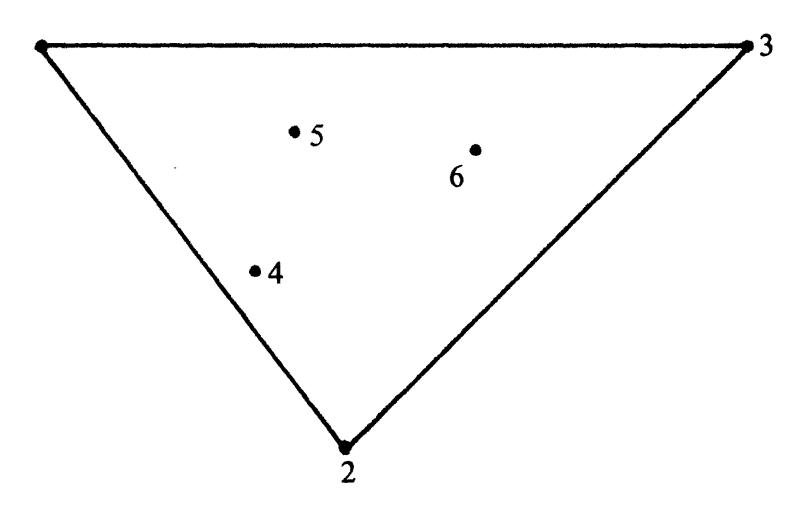
\includegraphics[scale=0.5]{images/geometric_approach_angle1.png}
	\caption{Οι "εσωτερικές" πόλεις είναι τα σημεία με label 4,5 και 6. Οι "εξωτερικές" πόλεις βρίσκονται στο convex hull (partial μονοπάτι)\\ πηγή: \cite{16}}
\end{matlab} 

\begin{matlab}
	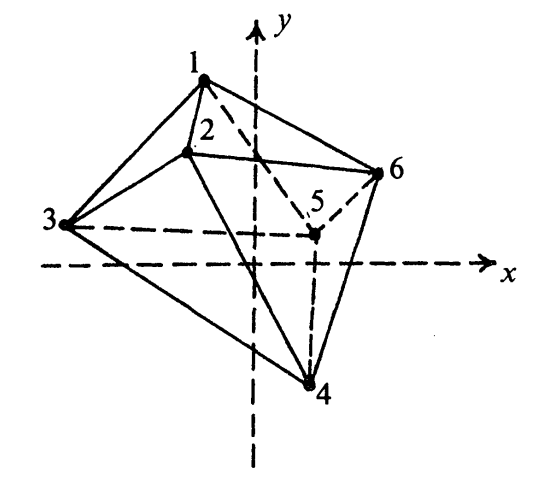
\includegraphics[scale=0.5]{images/geometric_approach_angle2.png}
	\caption{Στο σημείο αυτό έχει κατασκευαστεί το convex hull που αποτελείται από τέσσερα σημεία. Επίσης, έχουν κατασκευαστεί οι αντίστοιχες τέσσερεις γωνίες για κάθε μία από τις δύο εσωτερικές πόλεις. \\ πηγή: \cite{16}}
\end{matlab} 

\begin{matlab}
	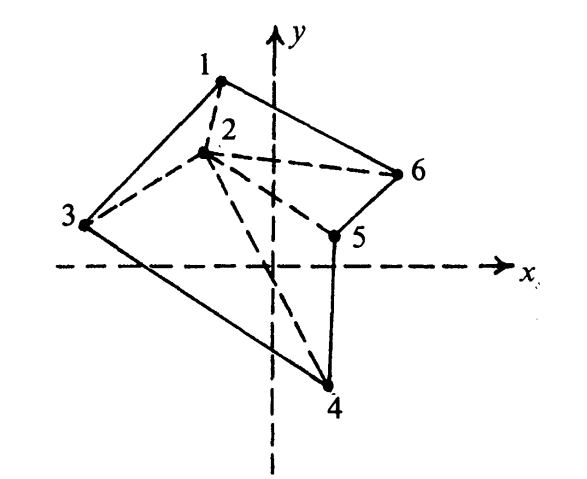
\includegraphics[scale=0.5]{images/geometric_approach_angle3.png}
	\caption{Η μεγαλύτερη γωνία από τις οκτώ που κατασκευάστηκαν ανήκει στο σημείο 5 και γι' αυτόν τον λόγο το σημείο 5 ενσωματώνεται στο partial μονοπάτι. \\ πηγή: \cite{16}}
\end{matlab} 

\begin{matlab}
	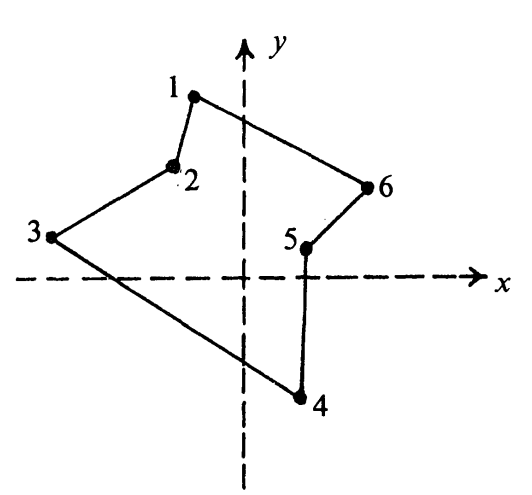
\includegraphics[scale=0.5]{images/geometric_approach_angle4.png}
	\caption{Κατασκευάζονται οι πέντε γωνίες γωνίες για το σημείο 2 και μιας που είναι και το τελευταίο σε αυτό ανήκει η μεγαλύτερη γωνία. Ενσωματώνεται για τον λόγο αυτό στο  μονοπάτι, που πλέον είναι ολοκληρωμένο. \\ πηγή: \cite{16}}
\end{matlab} 

Να αναφέρουμε στο σημείο αυτό, ότι ο εν λόγω αλγόριθμος δεν παράγει οπωσδήποτε το βέλτιστο μονοπάτι για το πρόβλημα του πλανόοδιου πωλητή κάθε φορά. Υπάρχουν περιπτώσεις, όπως αυτή που φαίνεται στην εικόνα 7.5, όπου ο αλγόριθμος αυτός δεν παράγει το βέλτιστο μονοπάτι, δηλαδή μπορεί να κατασκευάστει καλύτερο μονοπάτι, μονοπάτι στο οποίο ο πλανόδιος πωλητής θα διανύσει μικρότερη απόσταση. \\

\begin{matlab}
	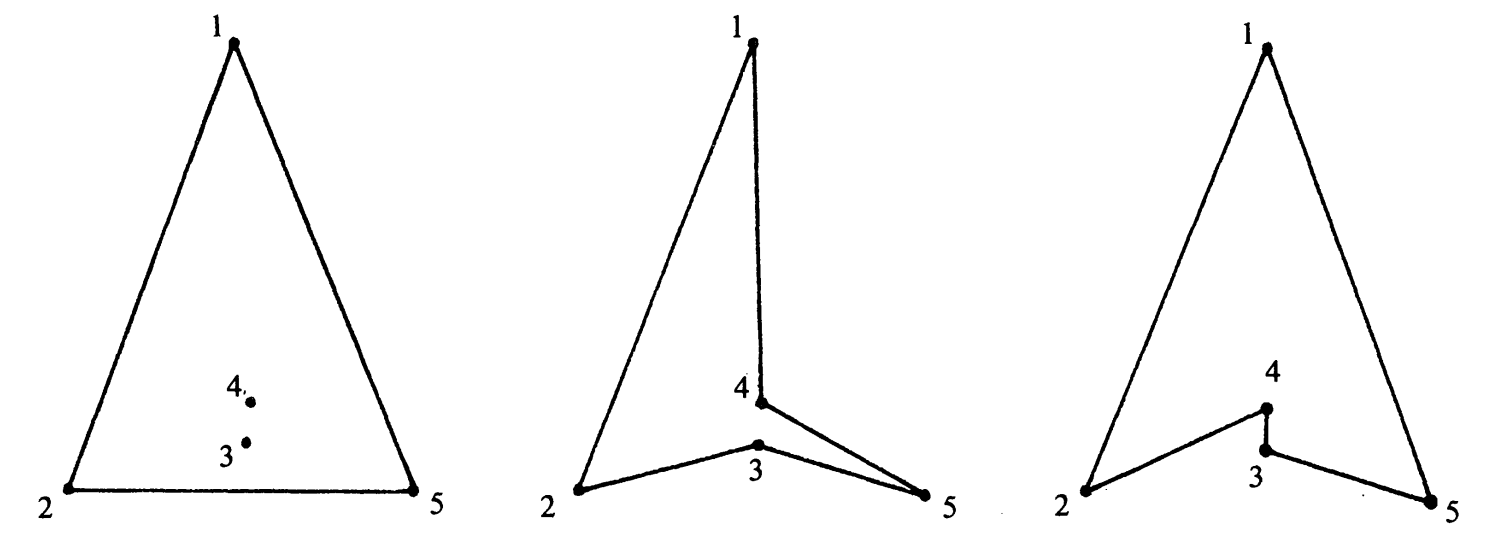
\includegraphics[scale=0.3]{images/geometric_approach_angle5.png}
	\caption{Παράδειγμα παραγωγής μη βέλτιστου μονοπατιού. Ο αλγόριθμος δίνει το αποτέλεσμα που φαίνεται στη μέση, ενώ το βέλτιστο αποτέλεσμα φαίνεται στα δεξία.\\ πηγή: \cite{16}}
\end{matlab} 

\subsection{Δεύτερη Γεωμετρική Προσέγγιση: Σύγκριση Ελλείψεων} 

Η δεύτερη γεωμετρική προσέγγιση απαιτεί και πάλι σε πρώτη φάση την εύρεση του convex hull, το οποίο και θεωρεί ως το partial μονοπάτι. Το επόμενο βήμα του αλγορίθμου είναι να εντοπίσει τη σειρά με την οποία θα ενσυματωθούν τα εσωτερικά σημεία στο μονοπάτι. Όπως και στον προηγούμενο αλγοριθμο σε κάθε επανάληψη του αλγορίθμου ενσωματώνεται μόνο μία καινούρια "εσωτερική" πόλη στο μονοπάτι και ο αλγόριθμος τερματίζει όταν όλες οι "εσωτερικές" πόλεις περιέχονται στο μονοπάτι του πλανόδιου πωλητή. \\

Ωστόσο, στον αλγόριθμο αυτό η επιλογή της πόλης που θα ενσωματωθεί στο partial μονοπάτι δε γίνεται με βάση τη μεγαλύτερη γωνία. Εδώ χρησιμοποιείται ως στοιχείο - κλειδί η έλλειψη. Πιο συγκεκριμένα, σε κάθε επανάληψη του αλγορίθμου δημιουργούνται όλες οι ελλείψεις που έχουν εστίες δύο διαδοχικά σημεία του convex hull και βαίνουν από ένα εσωτερικό σημείο. Για κάθε μία από τις ελλείψεις αυτές υπολογίζεται η εκκεντρότητά της. Η εκκεντρότητα για μία έλλειψη δίνεται από τον τύπο

\begin{align*}
	e = \frac{d_3}{d_1 + d_2}
\end{align*}

όπου \(d_3\) είναι η απόσταση μεταξύ των δύο εστιών και \(d_1, d_2\) είναι η απόσταση μεταξύ ενός σημείου της έλλειψης και των δύο εστιών αντίστοιχα, όπως φαίνεται στην εικόνα 7.6. \\

\begin{matlab}
	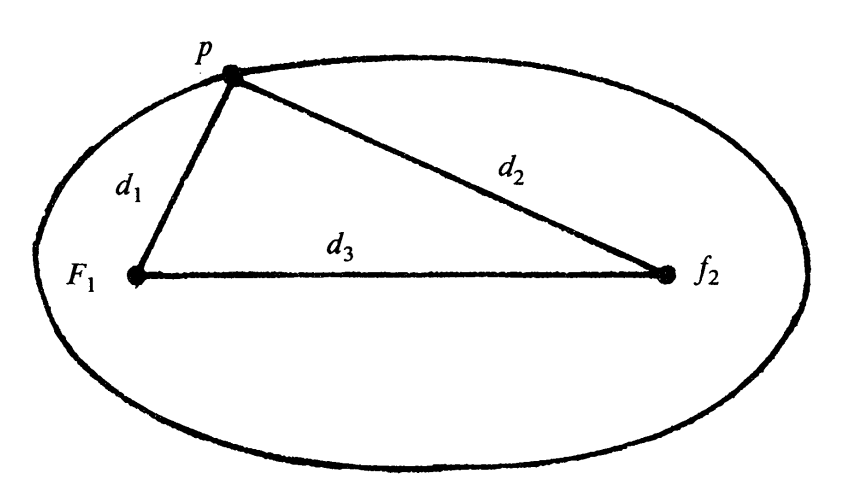
\includegraphics[scale=0.3]{images/geometric_approach_ellipse1.png}
	\caption{Η εκκεντρότητα δίνεται από τον τύπο \(e = \frac{d_3}{d_1 + d_2}\)\\ πηγή: \cite{16}}
\end{matlab}
 
 Ως επόμενο σημείο για το partial μονοπάτι επιλέγεται το σημείο εκείνο που ανήκει στην έλλειψη με τη μεγαλύτερη εκκεντρότητα (λιγότερο κυκλική μορφή). Ένα στιγμιότυπο του αλγορίθμου για ένα συγκεκριμένο παράδειγμα δίνεται στην εικόνα 7.7 και ο αλγόριθμος συνοψίζεται παρακάτω. \\
 
\begin{matlab}
  	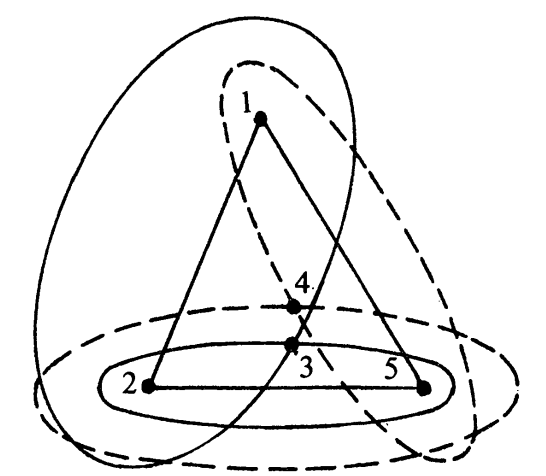
\includegraphics[scale=0.3]{images/geometric_approach_ellipse2.png}
	\caption{Στη φάση αυτή επιλέγεται το εσωτερικό σημείο με label 3, διότι ανήκει στην έλλειψη με τη μεγαλύτερη εκκεντρότητα.\\ πηγή: \cite{16}}
\end{matlab}  

\begin{algorithm}[H]
	\SetAlgoLined
	\KwIn{Σύνολο σημείων s στον Ευκλείδιο χώρο}
	\KwResult{Μονοπάτι για το TSP}
	
	partial\_tour = Κατασκεύασε το convex hull των σημείων της εισόδου \;
	out\_points = Σημεία που βρίσκονται στο convex hull \;
	in\_points = s - out\_points \;
	
	\While{in\_points \(\neq \emptyset\)}
	{
		\For{i} 
		{
			Κατασκεύασε όλες τις ελλείψεις με εστίες δύο διαδοχικά σημεία του partial\_tour που βαίνουν από το σημείο in\_points[i] \; 
			Υπολόγισε την εκκεντρότητα όλων των ελλείψεων και αποθήκευσε τη μεγαλύτερη από αυτές \;
		}
		partial\_tour = Επέλεξε το εσωτερικό σημείο που ανήκει στην έλλειψη με τη μεγαλύτερη εκκεντρότητα συνολικά \;
	}
	
	\caption{Εύρεση μονοπατιού TSP με βάση την εκκεντρότητα ελλείψεων}
\end{algorithm}

\subsection{Τρίτη Γεωμετρική Προσέγγιση: τριγωνοποίηση Delaunay}

Ένας από τους πλέον διαδεδομένους γεωμετρικούς τρόπους προσέγγισης του προβλήματος του περιοδεύοντος πωλητή είναι η προσέγγιση με βάση την τριγωνοποίσηση Delaunay. Έχουμε αναφερθεί εκτενώς στην τριγωνοποίηση Delaunay στο αντίστοιχο κεφάλαιο που αφορά το απαραίτητο μαθηματικό υπόβαθρο για την κατανόηση της παρούσας μελέτης. \\

Η τριγωνοποίηση Delaunay έχει μερικά χαρακτηριστικά τα οποία μπορούν να φανούν ιδιαιτέρως σημαντικά στο πρόβλημα του πλανόδιου πωλητή. 

\begin{itemize}
	\item Μεγιστοποιεί τη μικρότερη γωνία των τριγώνων της τριγωνοποίησης.
	\item Μπορεί να υπολογιστεί σε χρόνο \(Ο(n \log(n))\).
	\item Για κάθε τρίγωνο της τριγωνοποίησης υπάρχει κύκλος που περιέχει τις τρεις κορυφές του τριγώνου και μόνο αυτές.
	\item Είναι μοναδική αν δεν υπάρχουν τέσσερα σημεία που βρίσκονται στον ίδιο κύκλο.
	\item Περιέχει proximity graphs όπως το MST, το nearest neighbor graph, relative neighbor graph, Gabriel graph.
\end{itemize}

Η Delaunay τριγωνοποίηση μπορεί να συμβάλλει στην εύρεση μιας κατάλληλης διαδρομής για τον πλανόδιο πωλητή. Ωστόσο, δεν είναι απαραίτητο ότι θα καταφέρει να εντοπίσει την βέλτιστη διαδρομή, δηλαδή τη διαδρομή εκείνη που ελαχιστοποιεί το συνολικό κόστος, με άλλα λόγια τη συνολική απόσταση που χρειάζεται να διανύσει ο πωλητής. Υπάρχουν περιπτώσεις, όπου οι αλγόριθμοι επίλυσης του TSP με τη βοήθεια της Delaunay τριγωνοποίησης δεν παράγουν το βέλτιστο μονοπάτι. Το βέλτιστο μονοπάτι δεν είναι πάντοτε ένα υποσύνολο του Delaunay γράφου. Ένα τέτοιο παράδειγμα φαίνεται στην εικόνα 5.1. Ωστόσο, η Delaunay τριγωνοποίηση μπορεί να δώσει μία αρκετά καλή προσέγγιση της λύσης του προβλήματος. \\

Στην υποενότητα αυτή παρουσιάζουμε έναν αλγόριθμο εύρεσης μονοπατιού για το πρόβλημα του πλανόδιου πωλητή με βάση την Delaunay τριγωνοποίηση όπως παρουσιάζεται στο \cite{10}. \\

\begin{matlab}
	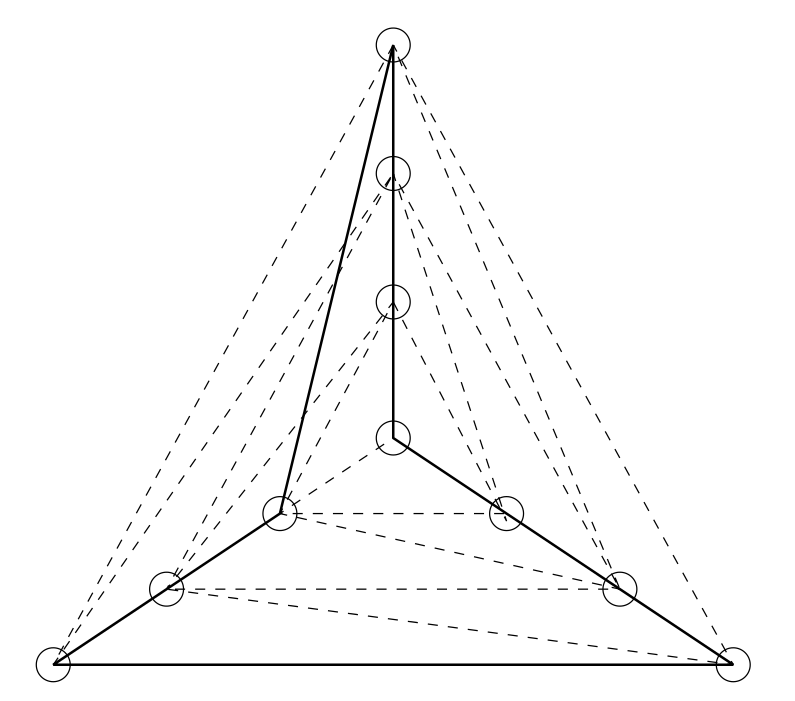
\includegraphics[scale=0.5]{images/delaunay_optimum_tour.png}
	\caption{Η καλύτερη διαδρομή δεν είναι στο υποσύνολο του Delaunay γράφου \\ πηγή: "An O(n log n) Heuristic for the Euclidean Traveling Salesman Problem" \cite{10} }
\end{matlab} 

Πρωτού ξεκινήσει η διαδικασία κατασκευής της διαδρομής, οι πόλεις, που πλέον λογίζονται ως σημεία στο επίπεδο, πρέπει να έχουν περάσει από τη διαδικασία της τριγωνοποίησης Delaunay. Έπειτα, από την τριγωνοποίηση των σημείων ο αλγόριθμος έχει να διαχείριστεί έναν γράφο, όπου οι πόλεις είναι οι κόμβοι του γράφου και οι διαδρομές (οι ακμές που έχουν παραχθεί από την τριγωνοποίηση) είναι οι ακμές του γράφου. Ο αλγόριθμος ξεκινά με μία διαδρομή \(T_i\) που περιέχει κάποιες από τις πόλεις σταθμούς και \(i\) το πλήθος ακμές που υποδεικνυουν την διαδρομή. Επιχειρεί με επαναλαμβανόμενα βήματα να εντάξει και τις υπόλοιπες. \\

Στο σημείο αυτό αναφέρουμε τον απαραίτητο συμβολισμό για την περαιτέρω ανάλυση του αλγορίθμου. \\

\begin{align*}
	& \bullet \text{ } E_{mn} \text{ είναι η ακμή που συνδέει τις πόλεις } C_m, C_n \\
	& \bullet \text{ } C_L(E_{mn}) \text{ είναι η πόλη που βρίσκεται στο αριστερό τρίγωνο της } E_{mn} \\
	& \bullet \text{ } C_R(E_{mn}) \text{ είναι η πόλη που βρίσκεται στο δεξί τρίγωνο της } E_{mn}
\end{align*}

Είναι προφανές πως κάθε ακμή του γράφου βρίσκεται ανάμεσα σε δύο τρίγωνα, εκτός αν πρόκειται για ακμή που βρίσκεται στο convex hull των σημείων. \\

Σε κάθε βήμα του αλγορίθμου μία από τις ακμές του \(T_i\) διαγράφεται και στη θέση της εισάγονται δυο κανούριες ακμές. Έστω πως η ακμή που διαγράφεται είναι η \(E_{mn}\), που συνδέει τις πόλεις \(C_m\) και \(C_n\). Οι δύο νέες ακμές που προσθέτονται στό \(Τ_{i+1}\) είναι οι \(E_{mL}\) και \(E_{Ln}\), που συνδέουν την πόλη \(C_m\) με την πόλη \(C_L(E_{mn})\) και την πόλη \(C_L(E_{nm})\) με την πόλη \(C_n\). Ως \(E_{nm}\) λογίζεται η ακμή \(E_{mn}\), αλλά με αντίθετη φορά. Ευκολά μπορεί, λοιπόν κανείς να συμπεράνει ότι \(C_L(E_{mn}) = C_L(E_{nm})\) Φυσικά, το βήμα αυτό λαμβάνει χώρα μόνο εαν η \(C_L(E_{mn})\) δεν ανήκει στις πόλεις που ήδη περιέχονται στη διαδρομή του πλανόδου πωλητή στο βήμα \(T_i\). Δίνεται ο αλγόριθμος Remove Edge, που υλοποιεί τη διαγραφή ακμής και την εισαγωγή δύο νέων ακμών παρακάτω. Θα μπορούσαμε αντίστοιχα να αναφερθούμε και στην πόλη \(C_R(E_{mn})\), ωστόσο κατί τέτοιο είναι πλήρως αντίστοιχο με την αναφορά στην πόλη που βρίσκεται στα αριστερά, οπότε o αλγόριθμος περιορίζεται μόνο στις πόλεις αυτές. Αφού, λοιπόν, ο αλγόριθμος επεκτείνεται προς τις πόλεις που βρίσκονται στα αριστερά, μία εύλογη επιλογή για αρχική διαδρομή θα ήταν το convex hull των σημείων με CCW σειρά. \\

\begin{algorithm}[H]
	\SetAlgoLined
	\KwResult{Αντικατάσταση ακμής του μονοπατιού με 2 νέεο ακμές}
	
	Διέγραψε το top του heap Ε \;
	\(e_1\) = ακμή αριστερού τριγώνου \;
	\(e_2\) = ακμή αριστερού τριγώνου \;	
	\(v\) = κορυφή μεταξύ των \(e_1\), \(e_2\) \;
	Πρόσθεσε το v στο tour \;
	Πρόσθεσε τα \(e_1\), \(e_2\) στο Ε \;
	
	\caption{Remove Edge}
\end{algorithm}

Το ερώτημα τώρα είναι πως καθορίζεται η επιλογή της \(E_{mn}\). Μία ακμή επιλέγεται να διαγραφεί, έναντι των άλλων, σύμφωνα με την ποιότητά της. Η ποιότητα της ακμής \(E_{mn}\) συμβολίζεται με \(Q_{mn}\) (από το quality). Ο υπολογισμός του μεγέθους \(Q_{mn}\) δεν έγκειται σε μία καθορισμένη διαδικασία. Μερικές προτεινόμενες προσεγγίσεις δίνονται παρακάτω. Θεωρούμε \(C_l = C_L(E_{nm})\) και \(L_i\) το μήκος της ακμής \(i\). \\

\begin{align*}
	& \bullet \text{ Farthest insertion} &&: Q_{mn} = - min(L_{ml}, L_{ln}) \\
	& \bullet \text{ Nearest insertion} &&: Q_{mn} = min(L_{ml}, L_{ln}) \\
	& \bullet \text{ Cheapest insertion} &&: Q_{mn} = -L_{ml} + L_{ln} - L_{mn} 
\end{align*}  

Σε μία κατάλληλη δομή δεδομένων φυλάσσονται τα qualities των ακμών, ώστε να μπορεί να γίνει η επιλογή της κατάλληλης ακμής προς διαγραφή. Μία τέτοια δομή είναι το heap. \\

Μετά την εκτέλεση των παραπάνω βημάτων είναι πολύ πιθανό να υπάρχουν πόλεις οι οποίες να μην περιλαμβάνονται ακόμα στο μονοπάτι του πλανόδιου πωλητή. Σε αυτήν την περίπτωση πρέπει να υπάρξει ειδική μέριμνα. Έστω ότι η πόλη που δεν ανήκει στο μονοπάτι μετα την εκτέλεση του αλγορίθμου είναι η \(C_x\). Τότε σίγουρα η \(C_x\) θα είναι γειτονική με κάποια άλλη πόλη, έστω τη \(C_m\). Επιλέγεται για διαγραφή η ακμή \(E_{mn}\) και προστίθονται οι ακμές \(E_{mx}\) και \(E_{xn}\). Αν υπάρχουν πολλές επιλογές για την επιλογή ακμής προς διαγραφή, τότε επιλέγεται εκείνη που ελαχιστοποιεί την αύξηση του τελικού μονοπατιού (\(L_{mx} + L_{xn} - L_{mn}\)). Να σημειωθεί εδω ότι η ακμή \(E_{xn}\) δεν είναι απαραίτητο να είναι ακμή της τριγωνοποίησης. \\

Ο υπορουτίνα που υλοποιεί την παραπάνω διαδικασία ονομάζεται Tour Finish. \\

\begin{algorithm}[H]
	\SetAlgoLined
	\KwResult{Ενσωμάτωση των πόλεων που δεν περιλαμβάνονται ακόμα στο μονοπάτι}
	
	Τοποθέτησε όλες τις πόλεις που δεν έχουν ακόμα ενσωματωθεί στο μονοπάτι σε ένα heap \;
	\For{πόλη c}
	{Αναζήτησε τις ακμές που μπορούν να χρησιμοποιηθούν για την εισαγωγή της πόλης \;
	\If{δεν υπάρχει κατάλληλη ακμή}
	{Τοποθέτησε την πόλη c στο heap \;
	continue \;}
	Διαγραφή ακμής \;
	Πρόσθεση 2 ακμών για την εισαγωγή της c \;}
	
	\caption{Tour Finish}
\end{algorithm}

Δύο βασικές βελτιώσεις στον αλγόριθμο που αναφέραμε είναι το clustering και το linear clustering. \\

Το cluestring αναφέρεται στα υπομονοπάτια που δημιουργούνται ξεκινόντας από το βασικό μονοπάτι (convex hull). Αν κατά τη διαδικασία αφαίρεση ακμής και εισαγωγής δύο νέων ακμών ο αλγόριθμος αποφασίσει πως αυτή του η ενέργεια είναι πιο δαπανηρή σε σχέση με τη δημιουργία μίας νέας υποδιαδρομής, τότε αλλάζει απόφαση και αντί να εκτελέσει το βασικό βήμα που περιγράψαμε παραπάνω δημιουργεί ένα ένα υπομονοπάτι, το οποίο καλείται cluster. Συνεπώς, ένα cluster είναι μία υποδιαδρομή, δηλαδή ένα σύνολο πόλεων που ενώνονται μεταξύ τους με ακμές. Το μικρότερο cluster που μπορεί να προκύψει αποτελείται από τρείς πόλεις, οι οποίες εννώνονται και δημιουργούν τρίγωνο. \\

Ο αλγόριθμος από την πρώτη στιγμή έχει γνώση των τριγώνων που έχουν δημιουργηθεί από την Delaunay τριγωνοποίηση και τα αποθηκέυει σε κατάλληλη δομή δεδομένων όπως θα δούμε παρακάτω. Κάθε τρίγωνο αξιολογείται για την ποιότητά του, όπως ακριβώς και οι ακμές από τον παρακάτω τύπο:

\begin{align*}
	Q_{t} = \frac{min(L_a, L_b, L_c)}{mid(L_a, L_b, L_c)}
\end{align*}

Μικρό \(Q_t\) σημαίνει ότι το τρίγωνο έχει μία πάρα πολύ μικρή γωνία και δύο πολύ μεγάλες σε μήκος ακμές. \\

Τα linear clusters είναι και αυτά clusters με τη διαφορά ότι δε δημιουργούν κύκλο, είναι απλά ένα μονοπάτι πάνω στον γράφο και η αρχική πόλη του μονοπατιού με την τελική δεν συμπίπτουν. \\

Παρακάτω παραθέτουμε τους αλγόριθμους που υλοποιούν τις διαδικασίες που σχετίζονται με τα clusters και τα linear clusters. \\

\begin{algorithm}[H]
	\SetAlgoLined
	\KwResult{Διαγραφή ακμής που ανήκει σε cluster και προσθήκη δύο νέων ακμών}
	
	Διέγραψε το top του heap C \;
	\(e_1\) = ακμή παρακείμενου τριγώνου \;
	\(e_2\) = ακμή παρακείμενου τριγώνου \;	
	\(v\) = κορυφή μεταξύ των \(e_1\), \(e_2\) \;
	Πρόσθεσε το v στο cluster \;
	Πρόσθεσε τα \(e_1\), \(e_2\) στο C \;
	
	\caption{Remove Cluster Edge}
\end{algorithm}

\begin{algorithm}[H]
	\SetAlgoLined
	\KwResult{Δημιουργία τριγώνου - cluster}
	
	Διέγραψε το top του heap T \;
	Δημιούργησε τρίγωνο \;
	Πρόσθεσε τις ακμές στο C \;
	
	\caption{Generate Cluster}
\end{algorithm}

\begin{algorithm}[H]
	\SetAlgoLined
	\KwResult{Δημιουργία linear cluster}
	
	\For{πόλη που δεν ανήκει στο tour}
	{Άνοιξε clusters με Delaunay ακμές \;
	Ενοποίησε την πόλη στο tour \;}
	
	\caption{Generate Linear Cluster}
\end{algorithm}

\newpage

\begin{algorithm}[H]
	\SetAlgoLined
	\KwResult{Ενοποίηση Cluster με Cluster ή CLuster με Tour}
	
	Διέγραψε το top του heap Μ \;
	\If{Cluster-Cluster}
	{Δίεγραψε 2 ακμές \;
	Προσθεσε 2 ακμές \;
	Προσθεσε τις ακμές στο C \;}
	\Else
	{Δίεγραψε 2 ακμές \;
	Προσθεσε 2 ακμές \;
	Προσθεσε τις ακμές στο Ε \;}
	
	\caption{Merge}
\end{algorithm}

Όπως είναι φανερό γίνεται εκτεταμένη χρήση της δομής heap. Πιο συγκεκριμένα χρησιμοποιείται ένα heap για τις ακμές του μονοπατιού και ένα heap Ε που θα φιλοξενήσει ακμές ταξινομημένες σύμφωνα με την ποιότητά τους (Q). Το Ε αρχικοποιείται με τις ακμές που convex hull των σημείων. Επίσης, χρησιμοποιείται ένα heap C, που περιέχει όλα τα clusters, ένα heap T, που περιέχει όλα τα τρίγωνα, ταξινομημένα σύμφωνα με την ποιότητα τους και ένα heap M, που περιέχει όλες τις πόλεις που προορίζονται για cluster merging. Παραθέτουμε τον βασικό αλγόριθμο που καλεί τις παραπάνω υπορουτίνες και υλοποιεί την ιδέα που αναπτύχθηκε στην αρχή της παρούσας ενότητας για την εύρεση μιάς καλής προσέγγισης του βέλτιστου μονοπατιού για τον πλανόδο πωλητή. \\

Η επιλογή της ενέργειας που θα εφαρμόσει σε κάθε βήμα ο αλγόριθμος γίνεται σύμφωνα με το κόστος που αυτή κατέχει (όπως ήδη έχουμε αναφέρει ενδεικτικά στην παράγραφο που αφορά τα clusters). Το κόστος αυτό υπολογίζεται από αντίστοιχες υπορουτίνες. \\

\begin{algorithm}[H]
	\SetAlgoLined
	\KwResult{Δημιουργία μονοπατιού}

	Υπολογισμός convex hull ;	
	Υπολογισμός Delaunay τριγωνοποίησης \;
	Υπολογισμός quality ακμών ;
	Υπολογισμός quality τριγώνων \;
	initial tour = convex hull \;
	Ε = ακμές του convex hull ;
	C = NULL ;
	T = τρίγωνα ;
	M = NULL \;
	\While{True}
	{edge cost = Edge Cost(E) ;
	cluster cost = Cluster Cost(C) \;
	triangle cost = Triangle Cost(T) ;
	merge cost = Merge(M) \;

	\If{egde cost \(>\) threshold and cluster cost \(>\) threshold}
	{break \;}
	
	\If{edge cost is best}
	{Remove Edge(E) \;
	continue \;}
	\If{cluster cost is best}
	{Remove Cluster Edge(C) \;
	continue \;}
	\If{triangle cost is best}
	{Generate Cluster(T) \;
	continue \;}
	\If{merge cost is best}
	{Merge(M) \;
	continue \;}}	

	Generate Linear Cluster() \;
	Tour Finish() \;
	
	\caption{TSP with Dealunay Triangulation}
\end{algorithm}

\newpage

\begin{algorithm}[H]
	\SetAlgoLined
	\KwResult{Yπολογισμός κόστους διαγραφής ακμής μονοπατιού}
	
	\(e\) = top του heap Ε \;
	\(e_1\) = ακμή παρακείμενου τριγώνου \;
	\(e_2\) = ακμή παρακείμενου τριγώνου \;	
	\(v\) = κορυφή μεταξύ των \(e_1\), \(e_2\) \;
	\If{v ανήκει στο μονοπάτι}
	{Κάλεσε ξανά τη διαδικασία \;}
	\If{v ανήκει σε cluster}
	{Υπολόγισε το κόστος για merge με το cluster \;
	Πρόσθεσε την e στο Μ \;
	Κάλεσε ξανά τη διαδικασία \;}
	Επέστρεψε το κόστος της e \;
	
	\caption{Edge Cost}
\end{algorithm}

\newpage

\begin{algorithm}[H]
	\SetAlgoLined
	\KwResult{Yπολογισμός κόστους διαγραφής ακμής cluster}
	
	\(e\) = top του heap C \;
	\(e_1\) = ακμή παρακείμενου τριγώνου \;
	\(e_2\) = ακμή παρακείμενου τριγώνου \;	
	\(v\) = κορυφή μεταξύ των \(e_1\), \(e_2\) \;
	\If{v ανήκει στο cluster}
	{\If{v ανήκει στο ίδιο cluster}
		{Κάλεσε ξανά τη διαδικασία \;}}
	Υπολόγισε κόστος merge με άλλο cluster \;
	Πρόσθεσε το ε στο Μ \;
	Κάλεσε ξανά τη διαδικασία \;
	\If{v ανήκει στο μονοπάτι}
	{Υπολόγισε το κόστος για merge με το μονοπάτι \;
		Πρόσθεσε την e στο Μ \;
		Κάλεσε ξανά τη διαδικασία \;}
	Επέστρεψε το κόστος της e \;
	
	\caption{Cluster Cost}
\end{algorithm}

\begin{algorithm}[H]
	\SetAlgoLined
	\KwResult{Yπολογισμός κόστους δημιουργίας τριγώνου}
	
	\(t\) = top του heap T \;
	\If{υπάρχει πόλη στο τρίγωνο που ανήκει σε cluster ή στο μονοπάτι}
	{Κάλεσε ξανά τη διαδικασία \;}
	Επέστρεψε το κόστος της e \;
	
	\caption{Triangle Cost}
\end{algorithm}

\chapter{Ειδικές Περιπτώσεις του Προβλήματος του πλανόδιου πωλητή}

Στην παρούσα ενότητα αναλύουμε ειδικά instances του προβλήματος του πλανόδιου πωλητή, τα οποία πρέπει να ικανοποιούν κάποιους επιπρόσθετους περιορισμούς ή έχουν κάποια ειδική δομή. \\

Στην πρώτη υποενότητα αναλύουμε το Convex Hull and Line TSP με βάση τη δημοσίευση \cite{17}, ενώ στη δεύτερη υποενότητα θα παρουσιάσουμε μία ευρέως γνωστή υποκατηγορία του γενικού TSP, που καλείται Time Window TSP, βασιζόμενοι στο \cite{1}. \\

\section{Convex Hull and Line TSP}

Σε αυτήν την υποενότητα θα αναφερθούμε σε μία ειδική κατηγορία του γενικού προβλήματος του πλανόδιου πωλητή, η οποία καλείται Convex Hull and Line TSP. \\

Πρόκειται για ένα στιγμιότυπο του προβλήματος του πλανόδιου πωλητή, όπου οι πόλεις που πρέπει να επισκεφτεί ο πωλητής είναι σημεία στον Ευκλείδιο χώρο. Αυτό σημαίνει πώς κάθε πόλη - σημείο χαρακτηρίζεται από δύο συντεταγμένες \((x,y)\), όπου \(x,y \in \R\) καθώς και ότι η απόσταση μεταξύ των σημείων υπολογίζεται με βάση την Ευκλείδια απόσταση. Τέλος, στον Ευκλείδιο χωρό ισχύει η τριγωνική ανισότητα. \\

Στο Convex Hull and Line TSP, που είναι μία ειδική περίπτωση του Ευκλείδιου TSP, οι πόλεις που πρέπει να επισκεφτεί ο πωλητής χωρίζονται σε δύο κατηγορίες. Η πρώτη κατηγορία περιέχει \(m\) το πλήθος πόλεις - σημεία τα οποία δημιουργούν ένα νοητό ευθύγραμμο τμήμα (δεν ικανοποιεί ακριβώς τα κριτήρια που ικανοποιεί ένα ευθύγραμμο τμήμα, ωστόσο εδώ θα χρησιμοποιούμε καταχρηστικά τον όρο αυτόν). Η δεύτερη κατηγορία απαρτίζεται από \(n\) το πλήθος πόλεις - σημεία τα οποία δημιουργούν ένα κυτό περίβλημα, που περιβάλλει τα \(m\) σημεία - πόλεις της πρώτης κατηγορίας (περισσότερες πληροφορίες σχετικά με το κυρτό περίβλημα και μία βασική θεωρία ο αναγνώστη μπορεί να βρεί στην αντίστοιχη υποενότητα του κεφαλαίου "Μαθηματικό Υπόβαθρο"). Παραθέτουμε ένα οπτικό παράδειγμα του Convex Hull and Line TSP στην αντίστοιχη εικόνα παρακάτω, για να γίνει πιο κατανοητό το πρόβλημα. \\

\begin{matlab}
	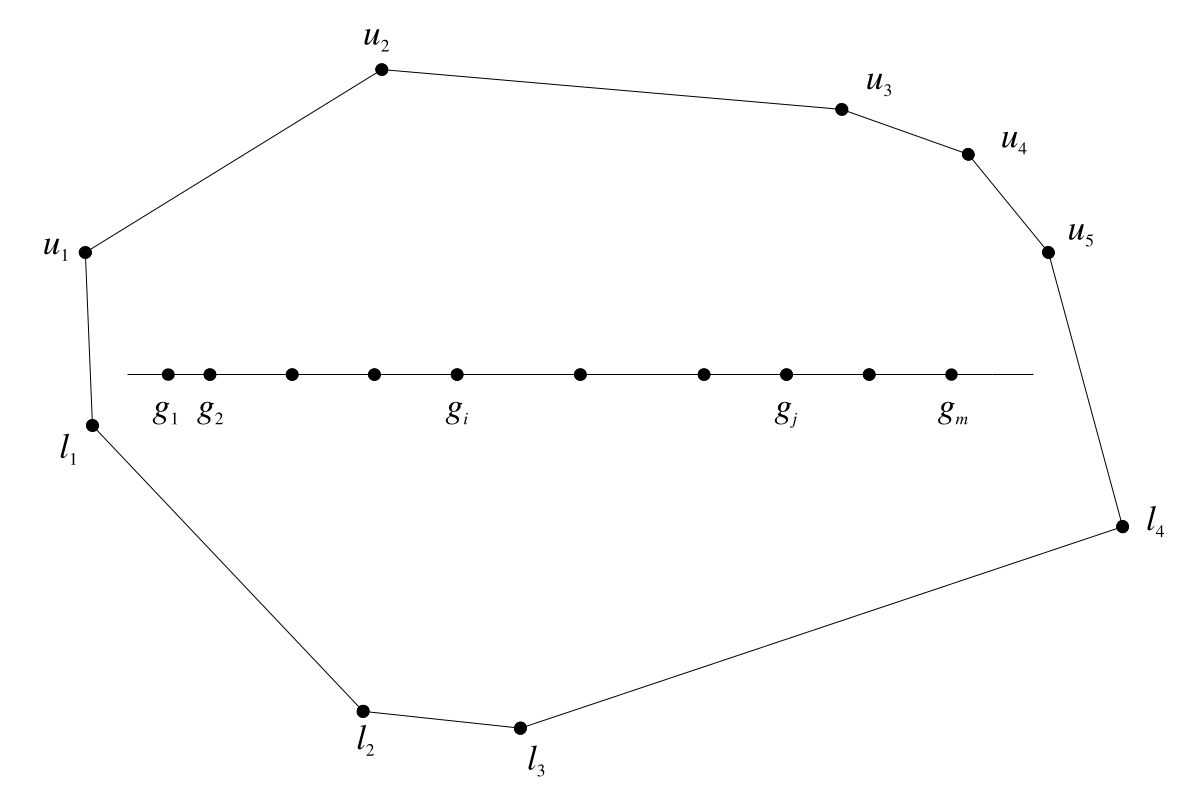
\includegraphics[scale=0.3]{images/ConvexHullLineTSP1.png}
	\caption{Οπτικό παράδειγμα ενός στιγμιοτύπου Convex Hull and Line TSP \\ πηγή: \cite{17}}
\end{matlab}   

\subsection{Συμβολισμός}

Στην παρούσα υποενότητα θα ακολουθήσουμε ένα συμβολισμό, ο οποίος είναι βασισμένος στο \cite{17}. Τα σημεία που ανήκουν στοευθύγραμμο τμήμα εντός του κυρτού περιβλήματος θα συμβολίζονται με \(g_i\), όπου \(1 \leq i \leq m\). Υποθέτουμε ότι \(m \geq 1\). Το σύνολο των σημείων \(\left\{g_1,...,g_m\right\}\) συμβολίζονται με \(G\). Επίσης, με \(G\) συμβλίζεται και η ευθεία που διέρχεται από τα σημεία \(\left\{g_1,...,g_m\right\}\). \\

Τα υπόλοιπα \(n\) σημεία, που βρίσκονται στο convex hull διακρίνονται σε δύο κατηγορίες. Τα σημεία που βρίσκονται πάνω από την ευθεία \(G\) και τα σημεία που βρίσκονται κάτω από αυτήν. Τα σημεία που βρίσκονται πάνω από την ευθεία \(G\) θα τα συμβολίζουμε με \(u_i\), για καταλληλο \(i\) ανάλογο με το πλήθος των σημείων και τα σημεία που βρίσκονται κάτω από την ευθεία \(G\) θα τα συμβολίζουμε με \(l_i\). Το σύνολο των σημείων που ανήκουν στο κυρτό περίβλημα θα συμβολίζεται με \(B\). \\

\subsection{Ανάλυση}

Στην περίπτωση του Ευκλείδιου TSP, μία πολύ σημαντική ιδιότητα είναι ότι το βέλτιστο μονοπάτι δεν διασταυρώνεται με τον εαυτό του. Η διαπίστωση αυτή μπορεί να θεμελιωθεί με αυστηρό τρόπο από το παρακάτω λήμμα. \\

\begin{mylemma}{}{}
	Έστω \(p,q,r,s\) τέσσερα σημεία στο επίπεδο που δημιουργούν ένα κυρτό τετράπλευρο με τη σειρά που δίνονται. Τρία από αυτά τα σημεία μπορούν να είναι συνευθειακά, αλλά όχι και τα τέσσερα. Στην περίπτωση αυτή ισχύει ότι 
	\(d(p,q) + d(r,s) < d(p,r) + d(q,s)\).
\end{mylemma}

Απόδειξη: \\
Το παραπάνω λήμμα υποδεικνύει ότι το άθροισμα των διαγωνίων του κυρτού τετραπλεύρου είναι μεγαλύτερο από το άθροισμα δύο πλευρώ του τετραπλεύρου. \\
Έστω \(v\) το σημείο που τέμνονται οι δύο διαγώνιες. Σχηματίζονται δύο τρίγωνα, το \(pvq\) και \(rvs\), για τα οποία ισχύει η τριγωνική ανισότητα

\begin{align}
	d(p,q) < d(p,v) + d(v,q) \\
	d(r,s) < d(r,v) + d(v,s)	
\end{align}

αντίστοιχα. Συνεπώς,

\begin{align}
	d(p,r) + d(q,s) = d(p,v) + d(v,r) + d(q,v) + d(v,s)
\end{align}

Αθροίζοντας τις (8.1) και (8.2) η (8.3) γίνεται

\begin{align*}
	d(p,r) + d(q,s) &= d(p,v) + d(v,r) + d(q,v) + d(v,s) \Rightarrow \\
	d(p,r) + d(q,s) &> d(p,q) + d(r,s)
\end{align*}

\(\square\)

Η βασική ιδέα εδώ είναι το μονοπάτι να ακολουθήσει μία "κυκλική" διαδρομή μίας κατεύθυνσης, ώστε να μην υπάρξουν πιθανές διασταυρώσεις και σε κατάλληλο σημείο, δηλαδή ανάμεσα σε δύο γειτονικές πόλεις του \(B\) να ενσωματωθούν οι πόλεις που ανήκουν στο σύνολο \(G\). Συνεπώς, το βασικό ζήτημα είναι να καθορίσουμε το σημείο στο οποίο θα ενσωματωθούν οι πόλεις που ανήκουν στο σύνολο \(G\). \\

\begin{mylemma}{}{}
	Έστω \(v,w \in B\) δύο γειτονικές πόλεις (δηλαδή δεν παρεμβάλλεται κάποια άλλη πόλη μεταξύ τους) και \(g_i, g_j \in G\). Αν στο βέλτιστο μονοπάτι οι πόλεις \(g_i, g_j\) βρίσκονται μεταξύ των πόλεων \(v,w\), τότε όλες οι πόλεις \(g_k \in G\) που βρίσκονται μεταξύ των \(g_i, g_j\) βρίσκονται στο μονοπάτι μεταξύ των πόλεων \(v,w\).
\end{mylemma} 

Απόδειξη: \\
Αν υπάρχει πόλη \(g_k \in G\) που βρίσκεται ανάμεσα στις πόλεις \(g_i, g_j \in G\) και δε βρίσκεται στο μονοπάτι ανάμεσα στις πόλεις \(v,w \in B\), τότε το μονοπάτι παρουσιάζει διασταύρωση και δεν είναι βέλτιστο. \(\square\)

Με βάση το λήμμα αυτό και το γεγονός ότι το μονοπάτι διέρχεται από τις πόλεις που βρίσκονται στο κυρτό περίβλημα με "κυκλική" σειρά προκύπτει το παρακάτω βασικό λήμμα. \\

\begin{mylemma}{}{}
	Σε ένα βέλτιστο μονοπάτι το σύνολο \(G\) μπορεί να διασπαστεί σε \(k+1\) υποσύνολα: \(\left\{g_1,...,g_{i_1}\right\}, \left\{{g_{i_1}}_{+1},...,g_{i_2}\right\},...,\left\{{g_{i_k}}_{+1},...,g_{m}\right\}\), όπου \(0 \leq k \leq m\) και \(0=i_0 < i_1 < ... < i_k < m\) και τα σύνολα αυτά να ενσωματωθούν το καθένα ανάμεσα σε δύο γειτονικές πόλεις του συνόλου \(B\).
\end{mylemma}

Στο σημείο αυτό προκύπτουν δύο βασικά ζητήματα. Το πρώτο έχει να κάνει με τον τρόπο που θα ενσωματωθεί καθένα από τα \(k+1\) υποσύνολα πόλεων που ανήκουν στο \(G\) στο μονοπάτι, δηλαδή το καθένα ανάμεσα σε δύο γειτονικές πόλεις που ανήκουν στο \(B\). Από όλους τους πιθανούς τρόπους πρέπει να επιλεγεί εκείνος που θα επιφέρει το καλύτερο δυνατό τελικό αποτέλεσμα, δηλαδή τη μικρότερη σε απόσταση διαδρομή για τον πλανόδιο πωλητή. Το δεύτερο ζήτημα σχετίζεται με τον τρόπο με τον οποίο πρέπει να χωριστούν σε \(k+1\) υποσύνολα οι πόλεις του \(G\). Από όλα τα πιθανά σύνολα υποσυνόλων θα πρέπει να επιλεγεί εκείνο που διαχωρίζει πιο αποτελεσματικά τις πόλεις του \(G\). \\

Θα αναφερθούμε αρχικά στο πρώτο ζήτημα. Δίνουμε τον παρακάτω ορισμό για τα σημεία \(v,w \in B\) και στη συνέχεια εξηγούμε αναλυτικά τον ευρύτερο συλλογισμό.

\begin{mydefinition}{Αποδεκτοί γείτονες}{}
	Δύο σημεία \(v,w \in B\) καλούνται αποδεκτοί γείτονες και μεταξύ τους μπορεί να παρεμβληθεί παράκαμψη μονοπατιού που πειέχει το σύνολο των πόλεων \(\left\{g_i,...,g_j\right\}\), όπου \(1 \leq i < j \leq m\) αρκεί να ισχύει μία από τις παρακάτω συνθήκες: \\
	1. Τα σημεία \(v,w\) βρίσκονται (και τα δύο) είτε πάνω από την ευθεία G, είτε κάτω από αυτήν ή \\
	2. \(\left\{v,w\right\} = \left\{u_p, l_p\right\}\) και \(j = m\) ή \\
	3. \(\left\{v,w\right\} = \left\{u_1, l_1\right\}\) και \(i = 1\) 
\end{mydefinition} 

Στο σημείο αυτό, πρέπει να αναλύσουμε λίγο παραπάνω την πρώτη συνθήκη του παραπάνω ορισμού. Έστω τα σημεία \((u_k, u_{k+1})\), με τέτοιο \(k\) ώστε κανένα από αυτά τα δύο αυτά σημεία να μην είναι ούτε το \(u_1\), όυτε το \(u_p\) και έστω ότι ανάμεσα στα δύο αυτά γειτονικά σημεία θέλουμε να παρεμβάλλουμε μονοπάτι που περιλαμβάνει το υποσύνολο \(\left\{g_i,...,g_j\right\}\) του συνόλου \(G\). Μπορεί κανείς εύκολα να παρατηρήσει πως είτε το μονοπάτι \(v,g_i,...,g_j, w\), είτε το μονοπάτι \(v,g_j,...,g_i,w\) διασταυρώνεται με τον εαυτό του. Στο παράδειγμα της εικόνας 8.1, λόγου χάρη, η διαστάυρωση αυτή προκύπτει στο μονοπάτι \(v,g_i,...,g_j, w\), αν υποθέσουμε ότι \(v = u_2\) και \(w = u_3\) ενδεικτικά. Το ίδιο ακριβώς συμβαίνει αν τα \(v,w\) βρίσκονται κάτω από την ευθεία G. Κατά συνέπεια, είναι σημαντικό να επισημαίνεται η σειρά με την οποία εισέρχονται οι πόλεις του συνόλου \(G\) στο μονοπάτι. \\ 

Στην περίπτωση που \(\left\{v,w\right\} = \left\{u_1, l_1\right\}\) η σειρά δεν παίζει καθοριστικό ρόλο, διότι δεν προκύπτει κανένα σημείο διασταύρωσης του μονοπατιού. Ωστόσο, αυτό που πρέπει να προσέχουμε στην περίπτωση αυτήν είναι το εξής: 

\begin{mylemma}{}{}
	Το υποσύνολο \(\left\{g_i,...,g_j\right\}\) του συνόλου \(G\) δε μπορεί να παρεμβληθεί μεταξύ των \(u_1\) και \(l_1\) σε ένα βέλτιστο μονοπάτι παραμόνο στην περίπτωση που το \(i = 1\). Παρομοίως, το ίδιο υποσύνολο πόλεων δεν μπορεί να παρεμβληθεί μεταξύ των \(u_p\) και \(l_p\) σε βέλτιστο μονοπάτι, παραμόνο στην περίπτωση που \(j = m\).
\end{mylemma}

Απόδειξη: \\
Έστω η περίπτωση όπου το \(i > 1\). Αυτό σημαίνει ότι το μονοπάτι \(u_1,g_i,...,g_j,l_1\) θα απομονώσει το σημείο \(g_1\) (ίσως και περισσότερα, αυτό εξαρτάται από το πόσο μεγάλο θα είναι το \(i\)) και με αυτό τον τρόπο οποιοδήποτε μονοπάτι προσπαθήσει να περάσει από το σημείο \(g_1\) θα χρειαστεί να διασταυρώσει το μονοπάτι \(u_1,g_i,...,g_j,l_1\), γεγονός που δεν επιτρέπεται αφού μιλάμε για κατασκευή βέλτιστου μονοπατιού, δηλαδή μονοπατιού που εξ ορισμού δε μπορεί να περιέχει διασταυρώσεις. \\
Με παρόμοιο τρόπο αποδεικνύεται και η περίπτωση των \(u_p\) και \(l_p\). \(\square\) \\ 

Όπως αναφέραμε προηγουμένως, η διαδικασία αυτή πρέπει να γίνει με τον βέλτιστο δυνατό τρόπο, δηλαδή με όσο το δυνατό μικρότερο κόστος. Για να το επιτύχουμε αυτό πρέπει να καθορίσουμε το κόστος εισαγωγής υποσυνόλου πόλεων του \(G\) στο μονοπάτι. Το κόστος δίνεται από τον παρακάτω τύπο 

\begin{align*}
	e^{v,w}_{ij} = \min \left\{ d(v,g_{i+1}) + d(g_{i+1},g_j) + d(g_j,w) - d(v,w), 
								d(v,g_j) + d(g_j,g_{i+1}) + d(g_{i+1},w) - d(v,w) \right\}
\end{align*}

όπου \(v,w \in B\) δύο αποδεκτοί γείτονες και \(\left\{g_{i+1},...,g_j\right\}\) υποσύνολο του \(G\) να είναι οι παρεμβαλόμενες πόλεις. Συνεπώς, το κόστος της φθηνότερης επιλογή δίνεται από τον τύπο 

\begin{align*}
	b_{ij} = \min \left\{ e^{v,w}_{ij} | \left\{ v,w \right\} \text{ είναι αποδεκτοί γείτονες για το υποσύνολο } \left\{g_{i+1},...,g_j\right\} \right\}
\end{align*}

Αφού καθορίσαμε τον τρόπο με τον οποίον μπορούμε να υπολογίσουμε το κόστος εισαγωγής υποσυνόλου σημείων του \(G\) στο βασικό μονοπάτι και να επιλέξουμε το μικρότερο δυνατό κόστος, μένει να αποσαφηνίσουμε με ποιον τρόπο μπορούμε να διαχωρίσουμε το σύνολο \(G\) σε κατάλληλα υποσύνολα. \\

Στόχος εδώ είναι να διαχωρίσουμε το σύνολο \(G = \left\{g_1,...,g_m\right\}\) σε κατάλληλα υποσύνολα. Καθώς δεν έχουμε περιορισμούς για τη μορφή των υποσυνόλων αυτών, καταλαβαίνει κανείς ότι το πλήθος των διαφορετικών συνδυασμών είναι αρκετά μεγάλο. Συνεπώς, αυτό που πράττουμε εδώ είναι η κατασκευή ενός κατευθυνόμενο ακυκλικού γράφου \(D\), ο οποίος έχει για κορυφές το σύνολο \(\left\{0,1,...,m\right\}\) και ακμές \((i,j)\) με βάρη \(b_{ij}\) για κάθε \(0 \leq i < j \leq m\). Οι πιθανοί διαχωρισμοί του συνόλου \(G\) σχετίζονται με τα μονοπάτια που υπάρχουν στον γράφο \(D\). \\

Θα γίνουμε περισσότερο κατατοπιστικοί παραθέτοντας ένα ενδεικτικό παράδειγμα. Έστω ο εξής διαχωρισμός 

\begin{align*}
	\left\{ \left\{ g_1,g_2,g_3 \right\}, \left\{ g_4,g_5 \right\}, \left\{ g_6 \right\}, \left\{ g_7,g_8,g_9, g_{10} \right\}\right\}.
\end{align*}

Ο γράφος που δίνεται στην εικόνα παρακάτω παρουσιάζει από όλες τις πιθανές ακμές, μόνο εκείνες του παραπάνω διαχωρισμού. Προφανώς οι ακμές αυτές συσχετίζονται με κάποιο βάρος \(b_{ij}\). Το μήκος του μονοπατιού αυτού αναπαριστά το ελάχιστο κόστος της συγκεκριμένης διάσπασης σε υποσύνολα.\\

\begin{matlab}
	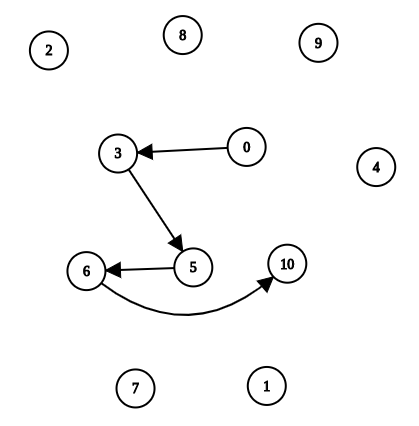
\includegraphics[scale=0.5]{images/graph.png}
	\caption{Αφαιρετικό παράδειγμα του γράφου. Φαίνονται μόνο οι ακμές του μονοπατιού της διαμέρισης \(\left\{ \left\{ g_1,g_2,g_3 \right\}, \left\{ g_4,g_5 \right\}, \left\{ g_6 \right\}, \left\{ g_7,g_8,g_9, g_{10} \right\}\right\}\) \\ πηγή: κατασκευάστηκε με τη βοήθεια του https://csacademy.com/app/graph\_editor/}
\end{matlab}

Συνεπώς, με βάση τον γράφο αυτόν και τα κόστη \(b_{ij}\) μπορούμε να αναζητήσουμε το μικρότερο σε συνολικό κόστος μονοπάτι με βάση τα βάρη των αντίστοιχων ακμών που ξεκινά από τον κόμβο 0 και καταλήγει στον κόμβο \(m\). Το μονοπάτι αυτό θα υποδείξει και τον καλύτερο δυνατό διαχωρισμό του συνόλου \(G\) σε υποσύνολα. \\

Αφού λοιπόν αναλύσαμε τα δύο βασικά ζητήματα της συγκεκριμένης προσέγγισης του Convex Hull and Line TSP μπορούμε να διατυπώσουμε το θεμελιώδες θεώρημα του προβλήματος. \\

\begin{mytheorem}{}{}
	Έστω \(σ\) ενα μονοπάτι που διέρχεται από τα σημεία που ανήκουν στο \(B\) με "κυκλική" φορά. Ένα μονοπάτι \(τ\) καλείται βέλτιστο αν και μόνο αν η εισαγωγή των σημείων του \(G\) στο \(σ\) γίνει με τέτοιον τρόπο, ώστε το αντίστοιχο μονοπάτι στον ακυκλικό κατευθυνόμενο γρράφο \(D\) έχει ελάχιστο μήκος. Το μονοπάτι \(τ\) έχει μήκος ίσο με το άθροισμα του μήκους του μονοπατιού \(σ\) και του αντίστοιχου μήκους στον γραφο \(D\). 
\end{mytheorem}

Απόδειξη: \\
...........................................

\subsection{Αλγόριθμος}

Στην υποενότητα αυτή παραθέτουμε τον αλγόριθμο του \cite{17} για το Convex Hull and Line TSP.  \\

Ο αλγόριθμος χωρίζεται σε δύο φάσεις. Στην πρώτη φάση υπολογίζεται το κόστος του καλύτερου μονοπατιού στο ακυκλικό κατευθυνόμενο γράφο \(D\). Στη δεύτερη φάση κατασκευάζεται το μονοπάτι για τον πλανόδιο πωλητή, με βάση το μονοπάτι του \(D\) που βρέθηκε στην πρώτη φάση. \\

Ο παρακάτω αλγόριθμος υπολογίζει τον καλύτερο διαχωρισμό των σημείων που ανήκουν στο \(G\). \\

\begin{algorithm}[H]
	\SetAlgoLined
	\KwIn{DAG D}
	\KwResult{Yπολογισμός κόστους βέλτιστου μονοπατιού του D}
	
	\(length_0 = 0\) \;
	\For{\(1 \leq j \leq m\)}
	{
		\For{\(0 \leq i \leq j-1\)}
		{
			Υπολόγισε το \(b_{ij}\) \;
			\(length_j = \min \left\{ length_i + b_{ij} \right\}\) \;
		}
	
		\(predecessor_j = \arg \min length_j\)
	}
	Επέστρεψε \(length_m \), predecessors
	
	\caption{Path Cost of D}
\end{algorithm}

Ο βασικός αλγόριθμος καλεί τον προηγούμενο αλγόριθμο και έπειτα κατασκευάζει το βέλτιστο μονοπάτι. \\

\begin{algorithm}[H]
	\SetAlgoLined

	\KwResult{Εύρεση βέλτιστου μονοπατιού για το Convex Hull and Line TSP}
	
	Path Cost of D \;
	
	j = m \;
	\While{\(j \neq 0\)}
	{
		\(i = predecessor_j\) \;
		Βρες αποδεκτούς γείτονες \(v,w\) για το υποσύνολο \(\left\{ g_{i+1},...,g_j \right\}\) τέτοιους ώστε \(b_{ij} = e^{v,w}_{ij}\) \;
		Τοποθέτησε τα \(\left\{ g_{i+1},...,g_j \right\}\) ανάμεσα στα \(v,w\) με την κατάλληλη σειρά \;
		j = i \;
	}
	Επέστρεψε \(length_m \)
	
	\caption{Convex Hull and Line TSP}
\end{algorithm}

\subsection{Χρονική και Χωρική Πολυπλοκότητα}

Η παραπάνω αλγοριθμική προσέγγιση έχει πολυπλοκότητα χρόνου \(Ο(mn)\) και πολυπλοκότητα χώρου \(Ο(n)\). \\

\begin{mytheorem}{Πολυπλοκότητα}{}
	Το Convex Hull and Line TSP με \(n\) το πλήθος πόλεις στο κυρτό περίβλημα και \(m\) το πλήθος πόλεις στο εσωτερικό ευθύγραμμο τμήμα χρειάζετα \(Ο(mn)\) χρονική πολυπλοκότητα και \(O(n)\) χώρο για να επιλυθεί.
\end{mytheorem}

Απόδειξη: \\
Αρχικά θα αναφερθούμε στην πρώτη φάση του αλγορίθμου, όπου εκτελείται ο αλγόριθμος Path Cost of D. Θα αποδείξουμε ότι για δεδομένο \(j\) και για κάθε \(0 \leq i < j\) το χρονικό κόστος για να εισαχθεί το \(\left\{g_{i+1},...,g_j\right\}\) μεταξύ των \(u_k\) και \(u_{k+1}\), όπου \(k = 1,...,p-1\) (και αντίστοιχα για \(l_k\) και \(l_{k+1}\)) είναι \(Ο(n)\). Αυτό σημαίνει ότι ο υπολογισμός \(b_{ij}\) απαιτεί \(Ο(n)\) χρόνο και κατά συνέπεια ο συνολικός χρόνος που απαιτείται από τον αλγόριθμος Path Cost of D είναι \(Οmn\). \\ 
θεωρούμε πίνακα Α με \(j\) το πλήθος γραμμές και \(p-1\) το πλήθος στήλες, όπου 

\begin{align*}
	a_{ik} = d(u_k, g_{i+1}) + d(g_{i+1}, g_j) + d(g_j,u_{k+1}) - d(u_k, u_{k+1})
\end{align*}

Αρκεί να βρούμε το ελάχιστο στοιχείο κάθε γραμμής. Έχει αποδειχτεί το 1987 από τον Aggarwal ότι όλα τα ελάχιστα γραμμών μπορούν να υπολογιστούν σε χρόνο \(Ο(j+p)\) αν ο πίνακας είναι μονότονος. Καθώς, για δεδομένο \(j\) χρειαζόμαστε στη μνήμη μόνο τα \(d_{ij}\), η φάση αυτή απαιτεί \(Ο(n)\) χώρο. \\
Η δεύτερη φάση του αλγορίθμου, όπου εντοπίζονται κατάλληλα \(v\) και \(w\) απαιτεί τον υπολογισμό του \(b_{ij}\), ο οποίος χρειάζεται \(Ο(n)\) χρόνο. Άρα συνολικά η δεύτερη φάση έχει \(Ο(mn)\) χρονική πολυπλοκότητα και \(Ο(n)\) χωρική πολυπλοκότητα.
Συνεπώς, ολόκληρος ο αλγόριθμος έχει \(Ο(mn)\) χρονική πολυπλοκότητα και \(Ο(n)\) χωρική πολυπλοκότητα. \(\square\) \\

\section{Time Window TSP}

Στην υποενότητα αυτή θα ασχοληθούμε με ένα ειδικό instance του προβλήματος του πλανόδιου πωλητή, το Time Window TSP. Η μελέτη μας βασίστηκε στο \cite{12}. \\

Ακόμα, θα αναφερθούμε σε ένα παρεμφερές πρόβλημα του Time Window TSP, το Time Window Prize Collecting. Αυτό κρίνεται σκόπιμο, διότι τα δύο προβλήματα κινούνται στην ίδια λογική και θα βοηθηθούμε στην ανάλυσή μας. Η προσέγγιση που ακολουθείται από το \cite{12} περιλαμβάνει και τα δύο προβλήματα, συνεπώς και εμείς θα παραμείνουμε πιστοί στη συγκριμένη ανάλυση. \\ 

Δυστυχώς, και το Time Window TSP και το Time WIndow Prize Collecting είναι NP-hard, διότι αποτελούν παραλλαγές του κλασσικού TSP. \\

\subsection{Time Window TSP} 

Το Time Window TSP (TWTSP) είναι μία υποκατηγορία του κλασσικού TSP, πρόκειται ουσιαστικά για το κλασσικό TSP μόνο που σε αυτήν την περίπτωση έχουν προστεθεί μερικές επιπλέον συνθήκες που πρέπει να ικανοποιούνται από το πρόβλημα . Κάθε σημείο επίσκεψης \(v\) χαρακτηρίζεται από ένα χρόνο deadline \(D(v)\) καί έναν χρόνο ελευθέρωσης (release time) \(R(v)\). Ο χρόνος ελευθέρωσης αναφέρεται στην χρονική στιγμή την οποία ξεκινά να είναι διαθέσιμο προς επίσκεψη το εκάστοτε σημείο, ενώ το deadline σηματοδοτεί το τέλος του επιτρεπτού χρόνου επίσκεψης του σημείου. Συνεπώς, κάθε σημείο επίσκεψης χαρακτηρίζεται από ένα time window \([R(v), D(v)]\). Ο πωλητής μπορεί να επισκεφτεί ένα σήμειο μόνο εντός του χρονικού πλαισίου \([R(v), D(v)]\). Στόχος στο TWTSP είναι να ελαχιστοποιηθεί η απόσταση που διανύεται από τον πωλητή, ο οποίος είναι υποχεωμένος να επισκεφτεί όλες τις πόλεις, την κάθε μία εντός του επιτρεπτού χρονικού πλαισίου. Θα συμβολίζουμε με \(λ*\) το μήκος του καλύτερου μονοπατιού \(P*\) στη βέλτιστη περίπτωση.  \\

\subsection{Time Window Prize Collecting}

Το Time Window Prize Collecting παρουσιάζει ομοιότητες με το Time Window TSP. Και σε αυτό το πρόβλημα κάθε πόλη χαρακτηρίζεται από ενα release time και ένα deadline. Στην περίπτωση, όμως, του TWPC ο πλανόδιος πωλητής δεν είναι υποχρεωμένος να επισκεφτεί όλες τις πόλεις, όπως είναι στην περίπτωση του TWTSP. Κάθε φορά που επισκέπτεται μία πόλη εντός του επιτρεπτού χρονικού διαστήματος, τότε λαμβάνει μία επιβράβευση. Εδώ στόχος είναι να μεγιστοποιηθεί η επιβράβευση που λαμβάνει ο πωλητής ή με άλλα λόγια να μεγιστοποιηθεί το πλήθος των πόλεων που έχει επισκεφτεί. Συνεπώς, στόχος είναι να βρεθεί ένα κατάλληλο μονοπατι με το οποίο να επιτυγχάνεται αυτή η μεγιστοποίηση. Θα συμβολίζουμε με \(k*\) το πλήθος των πόλεων που έχει επισκεφτεί ο πωλητής ακολουθώντας το μονοπάτι \(P*\) στη βέλτιστη περίπτωση. \\  

\subsection{Συμβολισμός}

Προτού προχωρήσουμε στη βαθύτερη ανάλυση θα εισάγουμε έναν στοιχειώδη συμβολισμό, που θα μας επιτρέψει να γίνουμε περισσότερο κατανοητοί στη συνέχεια. Και στην περίπτωση του TWTSP, αλλά και στην περίπτωση του TWPC θα μας απασχολήσει η ταχύτητα με την οποία κινείται ο πλανόδιος πωλητής. Στο εξής θα συμβολίζουμε την ταχύτητα με \(s\) και θα εξετάσουμε περιπτώσεις όπου η ταχύτητα αυτή είναι άπειρη και περιπτώσεις όπου η ταχύτητα αυτή είναι συγκεκριμένη. Θεωρούμε το σύνολο των πόλεων που πρέπει να επισκεφτεί ο πωλητής ως \(V = \left\{v_1, ..., v_n\right\}\) σημεία σε κάποιον χώρο. Η απόσταση μεταξύ δύο σημείων \(v_i\) και \(v_j\) συμβολίζεται με \(δ(v_i, v_j)\). Σε ό,τι αφορά τα release (\(r_i\)) και deadline (\(d_i\)) times για κάθε σημείο \(v_i\) θεωρούμε ότι ανήκουν στο διάστημα \([0,Τ]\), όπου \(Τ\) κάποιος θετικός ακέραιος αριθμός. Έστω \(L_i = d_i - r_i\) να είναι το μήκος του χρονικού παραθύρου του σημείου \(v_i\) και \(L_{max} = \max L_i\) να είναι το μέγεθος του μεγαλύτερου χρονικού παραθύρου. \\

Επίσης, εισάγουμε και κάποιους σημαντικούς ορισμούς. \\

\begin{mydefinition}{Δυαδικό time window}{}
	Ένα χρονικό παράθυρο (time window) \([r_i, d_i]\) καλείται δυαδικό αν το μήκος του ισούται με κάποια δύναμη του 2, δηλαδή \(L_i = 2^m\) για κάποιο ακέραιο \(m \geq 0\). Στην περίπτωση αυτήν, το \(r_i\) είναι ένας ακέραιος αριθμός πολλαπλάσιο του \(L_i\). 
\end{mydefinition}

\begin{mydefinition}{Δυαδικό στιγμιότυπο προβήματος}{}
	Κάθε στιγμιότυπο προβλήματος για το οποίο ισχύει ότι το \(L_i\) είναι δυαδικό \(\forall i \in [1,n]\), θα λέμε ότι είναι δυαδικό στιγμιότυπο προβλήματος. 
\end{mydefinition}

\begin{mydefinition}{Στοιχειώδες στιγμιότυπο προβήματος}{}
	Κάθε στιγμιότυπο προβλήματος για το οποίο ισχύει ότι: \\
	1. το time window \(\forall i \in [1,n]\) είναι μοναδιαίου μεγέθους, δηλαδή \( d_i - r_i = 1 \) \\
	ή είναι πλήρους μεγέθους, δηλαδη \([r_i, d_i] = [0,T]\) και \\
	2. \(\forall j \in [0,T-1], \exists\) τουλάχιστον ένα σημείο που έχει time window \([j, j+1]\) \\
	θα λέμε ότι είναι στοιχειώδες στιγμιότυπο προβλήματος. 
\end{mydefinition}

\subsection{Ανάλυση}

Παραθέτουμε μία εκτενή περιγραφή της προσέγγισης που μελετήσαμε. Αρχικά, αναλύουμε το πρόβλημα στη μία διάσταση, όπου δηλαδή οι πόλεις προς επίσκεψη ανήκουν σε μία ευθεία (ή παρομοίως σε μία καμπύλη). Στη συνέχεια εξατάζουμε το πρόβλημα στην γενικότερη μορφή του, όπου δηλαδή οι πόλεις εντοπίζονται σε κάποιον χώρο, όπου ισχύει κάποια μετρική, λόγω χάρη στον Ευκλείδιο χώρο, στον οποίο ισχύει η Ευκλείδια μετρική. \\

\subsection{TWTSP και TWPC σε 1 διάσταση}

Στην ενότητα αυτή να μελετήσουμε μία πιο απλή έκδοση των TWTSP και TWPC. Στην περίπτωση αυτήν οι πόλεις ή αλλιώς τα σημεία που πρέπει να επισκεφτεί ο πλανόδιος πωλητής είναι σημεία που ανήκουν σε μία ευθεία γραμμή ή μία καμπύλη γενικότερα. Θα δούμε δύο προσεγγίσεις αυτής της παραλλαγής. Στην πρώτη ο πωλητής μπορεί να ταξιδεύει από την μία πόλη στην άλλη με ταχύτητα \(s\), η οποία είναι άπειρη, ενώ στη δεύτερη περίπτωση η ταχύτητα θα είναι πεπερασμένη. \\

Οργανώνουμε τα δεδομένα χώρου (σημεία - πόλεις) και χρόνου (time windows) σε ένα σύστημα συντεταγμένων \(tx\). Ο οριζόντιος άξονας είναι ο άξονας \(t\) και σχετίζεται με τον χρόνο, ενώ ο κατακόρυφος άξονας \(x\) αφορά τις θέσεις των σημείων που πρέπει να επισκεφτεί ο πωλητής. Συνεπώς, τα time windows σε αυτήν την περίπτωση έχουν τη μορφή οριζόντιων ευθύγραμμων τμημάτων. Τα ευθύγραμμα τμήματα αυτά θα τα συμβολίζουμε σε \(σ_i\) για την πόλη \(v_i\). \\

.................. \\

\begin{mytheorem}{TWPC - 1D}{}
	Για ένα TWPC σε μία διάσταση με περιορισμένο όριο ταχύτητας \(s\) και \(L_{max}\) να είναι το μέγιστο μήκος ευθύγραμμου τμήματος \(σ\), υποθέτοντας ότι το μικρότερο time window έχει μήκος μεγαλύτερο ή ίσο με 1, τότε για οποιοδήποτε \(ε > 0\) μπορούμε να βρούμε μονοπάτι \(P\) σε χρόνο \(Ο((nL_{max})^{O(\frac{\log L_{max}}{\log 1 + ε})})\) τέτοιο ώστε: \\
	1. Το πλήθος των ευθυγράμμων τμημάτων που περιέχονται στο \(P\) να είναι τουλάχιστον όσα και στο βέλτιστο μονοπάτι και \\
	2. Ο πωλητής επισκέπτεται κάθε \(σ_i\) σε χρόνο \([r_i - εL_i, d_i + εL_i]\). 
\end{mytheorem}

Παρόμοια αποτελέσματα ισχύουν και για το TWTSP. \\

\subsubsection{Δυαδικά στιγμιότυπα με άπειρη ταχύτητα}

Η ανάλυση ξεκινά από μία ειδική κατηγορία στιγμιοτύπων του προβλήματος. Μελετάται η συμπεριφορά του TWTSP όταν τα time windows όλων των πόλεων είναι δυαδικά, δηλαδή το μήκος του αντίστοιχου ευθυγράμμου τμήματος είναι κάποια δύναμη του δύο, και η ταχύτητα του πλανόδιου πωλητή μπορεί να είναι άπειρη. Αυτο σημαίνει ότι πρακτικά η ταχύτητα δεν επιβάλλει κάποιον επιπλέον περιορισμό ως προς την επιλογή πόλης κάθε φορά, διότι η μετακίνηση από τη μία πόλη στην άλλη είναι πάντοτε εφικτή. \\

Αποδεικνύεται ότι δυαδικά στιγμιότυπα του προβλήματος μπορούν να επιλυθούν σε χρόνο \(n^{Ο(1)}\), όπου \(n\) είναι το πλήθος των σημείων προς επίσκεψη, αν η ταχύτητα με την οποία κινείται ο πωλητής είναι άπειρη. \\

\begin{mylemma}{TWTSP - 1D - \(s = \infty\)}{}
	Το TWTSP σε μία διάσταση με \(s = \infty\) για δυαδικά στιγμιότυπα του προβλήματος έχουν χρόνο επίλυσης \(poly(n) = n^{O(1)}\).
\end{mylemma}

Απόδειξη: \\
Η απόδειξη του λήμματος βασίζεται στον δυναμικό προγραμματισμό. \\
Έστω ότι με \(I = [a,b]\) συμβολίζουμε το χρονικό διάστημα μεταξύ της στιγμής \(a\) και \(b\), όπου το \(I\) είναι δυαδικό, σύμφωνα με τον ορισμό που έχει ήδη δοθεί. Με \(|P|\) συμβολίζουμε το μήκος του μονοπατιού \(P\). \\
Θεωρούμε το εξής πρόβλημα δυναμικού προγραμματισμου:

\begin{align*}
	&\min |P| \\
	&\text{ υπό τις προϋποθέσεις:} \\
	&\bullet \text{ Το μονοπάτι P να διέρχεται από όλα τα ευθύγραμμα τμήματα που βρίσκονται εντός του I} \\
	&\bullet \text{ Το σημείο με μέγιστη x-συντεταγμένη είναι το } x_N  \\
	&\bullet \text{ Το σημείο με ελάχιστη x-συντεταγμένη είναι το } x_S  \\	
	&\bullet \text{ Το μονοπάτι ξεκινά στο σημείο } x_b \\
	&\bullet \text{ Το μονοπάτι σταματά στο σημείο } x_e
\end{align*}

Με \(P^* = OPT(I;θ)\), όπου \(θ = (x_N, x_S, x_b, x_e)\) συμβολίζουμε τη βέλτιστη λύση. \\
Η μόνη περίπτωση όπου δεν είναι εφικτή η λύση είναι όταν το \(θ\) έχει οριστεί με τέτοιον τρόπο ώστε να μην είναι "λογικές" οι παράμετροί του. Τέτοιες περιπτώσεις είναι το σημείο με τη μέγιστη x-συντεταγμένη να είναι μικρότερο από το σημείο με την ελάχιστη x-συντεταγμένη, (\(x_N \leq x_S\)) ή το σημείο εκκίνησης για τον πωλητή να είναι μεγαλύτερο από το σημείο με τη μέγιστη συντεταγμένη \(x_b > x_N\). Σε τέτοιες περιτπώσεις το αποτέλεσμα ορίζεται να είναι \(- \infty\). \\
Χωρίζουμε το \(I\) σε δύο υποδιαστήματα, το \(I_L\) και \(I_R\), εντοπίζοντας το μέσο του \(I = [a,b]\), όπου με προφανές τρόπο είναι το σημείο \(\frac{a + b}{2}\). Το αριστερό υποδιάστημα είναι το \(I_L\) και το δεξί το \(I_R\). \\
Προφανώς, μπορούμε να εφαρμόσουμε το πρόβλημα δυναμικού προγραμματισμού και στα υποδιαστήματα \(I_L\) και \(I_R\). Η βέλτιστη λύση στην περίπτωση του αριστερού υποδιαστήματος θα είναι \(P^{*}_{I_L} = OPT(I_L;θ_L)\), όπου \(θ_L = (x_{N,L}, x_{S,L}, x_{b,L}, x_{e,L})\), όπου \(x_{N,L}\) είναι το σημείο με μέγιστη x-συντεταγμένη στο \(I_L\), \(x_{S,L}\) είναι το σημείο με ελάχιστη x-συντεταγμένη στο \(I_L\), \(x_{b,L}\) είναι η έναρξη του μονοπατιού για το \(I_L\) και \(x_{e,L}\) είναι ο καταληκτικός κόμβος του μονοπατιού για το διάστημα \(I_L\). Συμμετρικά ορίζεται και η βέλτιστη λύση για το υποδιάστημα \(I_R\). \\
Σε καθένα από τα υποδιαστήματα \(I_L\) και \(I_R\) υπάρχει μόνο ένα βέλτιστο μονοπάτι \(P^{*}_{I_L}\) και \(P^{*}_{I_R}\) αντίστοιχα και είναι μοναδικά, γιατί αν εξετάσουμε ενδεικτικά την περίπτωση του αριστερού υποδιαστήματος και υποθέσουμε ότι μπορεί να εντοπιστεί ένα ακόμα μονοπάτι \(P^{'}_{Ι_L}\) που να είναι βέλτιστο τότε η ένωση \(P^{*}_{Ι_L} \bigcap P^{'}_{Ι_L}\) θα είναι ένα μονοπάτι ακόμα πιο μικρό από ότι το βέλτιστο, γεγονός που δεν ισχύει έτσι όπως έχουμε παρουσιάσει την απόδειξη. \\
Η βέλτιστη λύση για το διάστημα \(Ι\) μπορεί να βρεθεί με βάση τις αντίστοιχες βέλτιστες λύσεις των αριστερών και δεξιών υποδιαστημάτων. Αν \(\max \left\{ x_{N,L}, x_{N,R} \right\} = x_N\), \(\min \left\{ x_{S,L}, x_{S,R} \right\} = x_S\) και \(x_{e,L} = x_{b,R}\), τότε

\begin{align*}
	OPT(I;θ) = \min \left\{ OPT\left\{ I_L;θ_L \right\} + OPT\left\{ I_R;θ_R \right\} \right\}
\end{align*}

Για ένα δεδομένο \(θ\) υπάρχουν \(O(n^4) \cdot O(n^4) = O(n^8)\) επιλογές για το \(θ_L\) και το \(θ_R\). Συνολικά υπάρχουν \(O(n^4)\) επιλογές για το \(θ\). Συνεπώς, η εύρεση του \(OPT(I,θ)\) χρειάζεται \(Ο(n^{12})\).........................................

Στη συνέχεια θα ορίσουμε μερικές καινούριες έννοιες. \\

\begin{mydefinition}{h-διαμέριση}{}
	Ένα διάστημα \([a,b]\) μπορεί να διαμεριστεί σε \(k \leq h\) υποδιαστήματα, υπό τη διαμέριση \(π: a = t_0 \leq t_1 \leq ... \leq t_{k-1} \leq t_k = b\)
\end{mydefinition}

\begin{mydefinition}{Σημείο Διαμέρισης}{}
	Κάθε \(t_i\) της διαμέρισης \(π: a = t_0 \leq t_1 \leq ... \leq t_{k-1} \leq t_k = b\) του διαστήματος \([a,b]\) καλείται σημείο διαμέρισης.
\end{mydefinition}

\begin{mydefinition}{Κληρονομική Ιδιότητα}{}
	Δοθέντος ενός συνόλου δυαδικών διαστημάτων, καθένα από τα οποία διαθέτει μία διαμέριση \(π\), λέμε ότι το σύνολο των διαμερίσεων έχουν την κληρονομική ιδιότητα αν για κάθε δύο \(I_1, I_2\) διαστήματα που είναι siblings, η ένωση των \(π(I_1)\) και \(π(I_2)\) είναι υπερσύνολο του \(π(Ι)\). 
\end{mydefinition}

\begin{mydefinition}{h-δυαδικό στιγμιότυπο προβλήματος}{}
	Κάθε στιγμιότυπο προβλήματος για το οποίο ισχύει ότι: \\
	1. Κάθε δυαδικό διάστημα \(I\) μπορεί να διαμεριστεί με το \(π(Ι)\), έτσι ώστε κάθε σύνολο διαμερίσεων να έχει την κληρονομική ιδιότητα.
	2. Τα άκρα κάθε ευθύγραμμου τμήματος \(σ_i\) είναι σημεία της διαμέρισης \(π(W(σ_i))\), όπου \(W(I)\) είναι τα ελάχιστα δυαδικά διαστήματα που περιέχει το \(I\). 
\end{mydefinition}

Αφού ορίσαμε τις παραπάνω έννοιες είμαστε σε θέση να επαναδιατυπώσουμε το πρόβλημα δυναμικού προγραμματισμού της προηγούμενη απόδειξης, έτσι ώστε να μπορεί να διαχειριστεί h-δυαδικά στιγμιότυπα προβλήματος. \\

Αν \(π\) είναι μία h-διαμέριση του \(I = [a,b]\) με σημεία διαμέρισης τα σημεία \(\left\{ t_i \right\}\) τότε το πρόβλημα επαναορίζεται ως εξής:

\begin{align*}
	&\min |P| \\
	&\text{ υπό τις προϋποθέσεις:} \\
	&\bullet \text{ Το μονοπάτι P να διέρχεται από όλα τα ευθύγραμμα τμήματα που βρίσκονται εντός του I} \\
	&\bullet \text{ Το σημείο με μέγιστη x-συντεταγμένη στο διάστημα } [t_{j-1}, t_j] \text{ είναι το } x^{j}_N  \\
	&\bullet \text{ Το σημείο με ελάχιστη x-συντεταγμένη στο διάστημα } [t_{j-1}, t_j] \text{ είναι το } x^{j}_S  \\
	&\bullet \text{ Το μονοπάτι ξεκινά στο σημείο } x_b \\
	&\bullet \text{ Το μονοπάτι σταματά στο σημείο } x_e
\end{align*}

\begin{mytheorem}{TWTSP - 1D - \(s = \infty\)}{}
	Το TWTSP σε μία διάσταση με \(s = \infty\) για h-δυαδικά στιγμιότυπα προβλήματος έχει χρόνο επίλυσης \(O(n^{O(h) \log L_{max}})\).
\end{mytheorem}

Απόδειξη:
Θεωρούμε ότι το διάστημα \(I\) είναι ο πατέρας των \(I_L\) και \(I_R\) και ότι τα διαστήματα αυτά έχουν h-διαμερίσεις \(π, π_L, π_R\) αντίστοιχα. Έστω με \(x(σ)\) να συμβολίζεται η χ συντεταγμένη ενός ευθύγραμμου τμήματος \(σ\). Αυτό που πρέπει να ισχύει στην περίπτωση του 1D TWTSP με h-διαμερίσεις είναι:

\begin{align*}
	OPT(I;π;θ) = \min \left\{ OPT(I_L;π_L;θ_L) + OPT(I_R;π_R;θ_R) \right\}
\end{align*}

υπό τις εξής προϋποθέσεις: \\
\begin{itemize}
	\item αν \(x\) είναι η ελάχιστη/μέγιστη συντεταγμένη που επισκέπτεται το \(P\) στο χρονικό διάστημα \([t_i, t_j]\), τότε το \(P\) διέρχεται από την \(x\) τουλάχιστον σε ένα υποδιάστημα του \(π_L\) ή του \(π_R\) στο \([t_i, t_j]\). 
\end{itemize}

\begin{align*}
	forall j \leq h \\
	x^{j}_N = \max \left\{ x^{i}_N: t_{j-1} \leq t_{i-1}^L \leq t_{i}^L \leq t_j \text{ ή } t_{j-1} \leq t_{i-1}^R \leq t_{i}^R \leq t_j \right\} \\
	x^{j}_S = \min \left\{ x^{i}_S: t_{j-1} \leq t_{i-1}^L \leq t_{i}^L \leq t_j \text{ ή } t_{j-1} \leq t_{i-1}^R \leq t_{i}^R \leq t_j \right\}
\end{align*}

\begin{itemize}
	\item Τα ευθύγραμμα τμήματα που περιέχονται στο \(V[t_i, t_j]\) περιέχονται όλα στο μονοπάτι \(P\) αν και μόνο αν η ένωση των κατακόρυφων ευρών του \(P\) στο διάστημα \([t_i, t_j]\) περιέχεται πλήρως στο κατακόρυφο εύρος του \(V[t_i, t_j]\)
\end{itemize}

\begin{align*}
forall i,j \leq h \\
\max \left\{ x^{i}_{N,L},...,x^{j}_{N,L}, x^{1}_{N,R},...,x^{j}_{N,R} \right\} \geq \max \left\{ x(σ): σ \in V[t_i, t_j] \right\} \\
\min \left\{ x^{i}_{S,L},...,x^{j}_{S,L}, x^{1}_{S,R},...,x^{j}_{S,R} \right\} \geq \max \left\{ x(σ): σ \in V[t_i, t_j] \right\}
\end{align*}

...................................

Τώρα είμαστε σε θέση να αναφερθούμε στην γενική περίπτωση του 1D TWTSP. \\
Πάλι η προσέγγιση χρησιμοποιεί h-διαμέριση. Η βασική ιδέα είναι κάθε δύαδικό διάστημα να υποστεί h-διαμέριση και έπειτα κάθε άκρο των ευθυγράμμων τμημάτων να μεταβληθεί ελαφρώς έτσι ώστε να συμπίπτει με σημείο της διαμέρισης \(π(W(σ))\), όπου \(W(σ)\) είναι το ελάχιστο δυαδικό διάστημα που περιέχει το σ. \\
Το κρίσιμο κομμάτι εδώ είναι να βρεθούν οι κατάλληλες διαμερίσεις. Πρέπει από τη μία τα σημεία της διαμέρισης να είναι αραιά, ώστε να περιορίσουμε την πολυπλοκότητα όμως παράλληλα πρέπει να είναι αρκετά πυκνά έτσι ώστε κάθε άκρο ευθύγραμμου τμήματος να μπορεί να ταυτιστεί με ένα σημείο διαμέρισης που δεν απέχει παρισσότερο από \((1+ε)\). \\

\begin{mydefinition}{ε-πυκνή διαμέριση}{}
	Έστω ένα διάστημα \(I = [a,b]\), όπου \(l = b - a\) και \(c = \frac{a+b}{2}\). Μία διαμέριση \(π\) καλείται ε-πυκνή αν: \\
	1. όλα τα σημεία διαμέρισης είναι ακέραιοι αριθμοί, \\
	2. είναι συμμετρική ως προς το c και \\
	3. \(\forall q \leq \log_{1+ε} l\) το υποδιάστημα \((1+ε)^q + a, (1+ε)^{q+1} + a\) περιέχει τουλάχιστον ένα σημείο διαμέρισης, εκτός αν δεν περιέχει κανένα σημείο ακέραιο.
\end{mydefinition}

\begin{mylemma}{ε-πυκνή διαμέριση με την ιδιότητα της κληρομικότητας}{}
	Έστω \(L_{max} > 0\) να είναι \(L_{max} = 2^m\) για κάποιο \(m \geq 0\) ακέραιο. Μία διαμέριση \(π(I)\) μπορεί να ανατεθεί σε κάθε δυαδικό διάστημα \(I \subseteq [0,L_{max}]\) αρκεί να ισχύουν τα παρακάτω: \\
	1. \(π(Ι)\) είναι μία οικογένεια διαμερίσεων με την ιδιότητα της κληρονομικότητας. \\
	2. κάθε \(π(Ι)\) έχει το πολύ \(Ο(\frac{\log L_{max}}{\log (1+ε)})\) σημεία. \\
	3. \(π(Ι)\) είναι ε-πυκνό \(\forall I \subseteq [0,L_{max}]\)
\end{mylemma}

Συνεπώς, τώρα μπορούμε να ναφερθούμε με αυστηρό τρόπο στο TWTSP στη μία διάσταση. \\

\begin{mytheorem}{TWTSP - 1D}{}
	Για ένα TWTSP σε μία διάσταση με όριο ταχύτητας \(s = \infty\) και \(L_{max}\) να είναι το μέγιστο μήκος ευθύγραμμου τμήματος \(σ\), για οποιοδήποτε \(ε > 0\) μπορούμε να βρούμε μονοπάτι \(P\) σε χρόνο \(Ο(n^{O(\frac{\log L_{max}}{\log 1 + ε})} \log L_{max})\) τέτοιο ώστε: \\
	1. Το μήκος του \(P\) να είναι το πολύ όσο το μήκος του βέλτιστου μονοπατιού και \\
	2. Ο πωλητής επισκέπτεται κάθε \(σ_i\) σε χρόνο \([r_i - εL_i, d_i + εL_i]\). 
\end{mytheorem}

Απόδειξη: \\
Κατασκευάζουμε μία ε-πυκνή διαμέριση και μετατρέπουμε το στιγμιότυπο του προλήματος σε h-δυαδικό στιγμιότυπο, με \(h = O(\frac{\log L_{max}}{\log (1+ε)})\). Κάθε άκρο των ευθυγράμμων τμημάτων μεταβάλλεται ελαφρώς έτσι ώστε να συμπίπτει με σημείο της διαμέρισης \(π(W(σ))\), όπου \(W(σ)\) είναι το ελάχιστο δυαδικό διάστημα που περιέχει το σ. Με χρήση του δυναμικού προγραμματισμού βρίσκει ένα μονομάτι P. Προφανώς, το P είναι μικρότερο σε μήκος σε σχέση με το βέλτιστο μονοπάτι. Το μονοπάτι διέρχετια από κάθε ευθύγραμμο τμήμα \(σ_i\) στο χρονικό παράθυρο \([r_i - εL_i, d_i + εL_i]\), επειδή έχουμε μετατοπίσει τα άκρα των ευθυγράμμων τμημάτων κατα \((1+ε)\) το πολύ. 

\subsubsection{Πεπερασμένη ταχύτητα}

Αν η ταχύτητα με την οποία κινείται ο πωλητής δεν είναι άπειρη (\(s < \infty\)), υπάρχει η πιθανότητα αν η ταχύτητα είναι εξαιρετικά μικρή να μην υπάρχει δυνατή λύση του προβλήματος. Αυτός είναι ο λόγος που στην περίπτωση αυτή αντί να χρησιμοποιηθεί το Time WIndow TSP, χρησιμοποιείται το Time Window Prize Collecting (TWPC). Εισάγουμε τον κατάλληλο συμβολισμό για τον ορισμό του προβλήματος δυναμικού προγραμματισμού στην περίπτωση όπου το \(s < \infty\). \\

Όπως και πριν το \(I = [a,b]\) συμβολίζει ένα δυαδικό διάστημα και το \(S(I)\) είναι το σύνολο των ευθυγράμμων τμημάτων τα οποία προβάλλονται στον άξονα του χρόνου και η προβολή βρίσκεται εντός του διαστήματος \([a,b]\). Με \(y_N\) συμβολίζεται η μεγαλύτερη συντεταγμένη στον άξονα του χώρου των ευθύγραμμων τμημάτων που περιλαμβάνονται στο μονοπάτι. Αντίστοιχα, με \(y_S\) συμβολίζεται η μικρότερη συντεταγμένη.Επίσης το τετράγωνο που ορίζεται από τα \(a,b\) και τα \(y_N, y_S\) συμβολίζεται με \(B(P,a,b)\), το άνω όριο του τετραγώνου συμβολίζεται με \(\partial^{N}(B)\) και αντίστοιχα το κάτω όριο με \(\partial^{S}(B)\). Με \(P(τ)\) θα συμβολόζεται η x-συντεταγμένη στην οποια βρίσκεται το μονοπάτι \(P\) την χρονική στιγμή \(τ\).

Το πρόβλημα δυναμικού προγραμματισμού στην περίπτωση αυτή δίνεται παρακάτω:

\begin{align*}
&\max \text{ πλήθος ευθυγράμμων τμημάτων που ανήκουν στο } S(I) \text{ που εντοπίζονται στο μονοπάτι } P \\
&\text{ υπό τις προϋποθέσεις:} \\
&\bullet \text{ Το σημείο με μέγιστη x-συντεταγμένη στο μονοπάτι } P \text{ εντός του } Ι \text{ είναι το } x_N  \\
&\bullet \text{ Το σημείο με ελάχιστη x-συντεταγμένη στο μονοπάτι } P \text{ εντός του } Ι \text{ είναι το } x_S  \\
&\bullet \text{ Το μονοπάτι ξεκινά στο σημείο } x_b \\
&\bullet \text{ Το μονοπάτι σταματά στο σημείο } x_e \\
&\bullet \text{ Το σημείο με μέγιστη x-συντεταγμένη στο μονοπάτι } P \text{ εντός του } S(I) \text{ είναι το } y_N  \\
&\bullet \text{ Το σημείο με ελάχιστη x-συντεταγμένη στο μονοπάτι } P \text{ εντός του } S(I) \text{ είναι το } y_S  \\
&\bullet τ_b = \min \left\{ τ \in [a,b] : P(τ) \in [y_S, y_N] \right\}  \\
&\bullet τ_e = \max \left\{ τ \in [a,b] : P(τ) \in [y_S, y_N] \right\}  \\
&\bullet \text{ Το μονοπάτι φτάνει στο } y_N \text{ την χρονική στιγμή } τ_{N}^{-} \text{ πηγαίνει στο } x_N \text{ και επιστρέφει στο } y_N \text{ την χρονική στιγμή } τ_{N}^{+} \\
&\bullet \text{ Το μονοπάτι φτάνει στο } y_S \text{ την χρονική στιγμή } τ_{S}^{-} \text{ πηγαίνει στο } x_S \text{ και επιστρέφει στο } y_S \text{ την χρονική στιγμή } τ_{S}^{+} 
\end{align*} 

Η βέλτιστη λύση σε αυτήν την περίπτωση είναι η \(OPT(I;θ)\), όπου \\ \(θ = (y_N, y_S; x_N, x_S; x;_b, x_e; τ_b, τ_e, τ_{N}^{-} ,τ_{N}^{+}, τ_{S}^{-}, τ_{S}^{-})\)

Ουσιαστικά το μονοπάτι πρέπει να περάσει από μερικά σημεία σταθμούς (\(x_b, y_N, y_S, x_e\)) στις αντίστοιχες χρονικές στιγμές όπως προκύπτουν από τους περιορισμούς που δόθηκαν παραπάνω δημιουργώντας μία "καμπύλη". Στόχος είναι να βρεθεί η καμπύλη εκείνη που μεγιστοποιεί το πλήθος των ευθυγράμμων τμημάτων εντός του \(S(I)\). Με αυτόν τον τρόπο ο πωλητής επισκέπτεται περισσότερες πόλεις και συνεπώς μεγιστοποιεί το κέρδος, καθώς αναφερόμαστε σε TWPC πρόβλημα. \\

\begin{mylemma}{TWPC - 1D}{}
	Το TWPC πρόβλημα σε μία διάσταση με δυαδικά παράθυρα χρόνου μπορεί να λυθεί σε χρόνο \(poly(n,L_{max})\)
\end{mylemma}

Απόδειξη: \\
....................................................

\subsection{TWTSP στο χώρο}

Μπορούμε πλέον να ασχοληθούμε με τη γενική περίπτωση, όπου οι πόλεις που πρέπει να επισκεφτεί ο πωλητής βρίσκονται σε κάποιον χώρο, όπου ισχύει μία μετρική \(δ\), όπως για παράδειγμα στον Ευκλείδιο χώρο, όπου ισχύει η Ευκλείδια απόσταση. \\

Υποθέτουμε σε αυτήν την περίπτωση ότι ο πωλητής μας μπορεί να κινείται με μία ταχύτητα \(s\) που ξεπερνά κάποιο threshold ταχύτητας \(s_{min}\). Αν η ταχύτητά του είναι μικρότερη από αυτήν, τότε θεωρούμε ότι το πρόβλημα δε μπορεί να έχει εφικτή λύση. \\

Θα συμβολίζουμε με \(λ^{*}(s)\) το βέλτιστο μονοπάτι, δηλαδή το μονοπάτι εκείνο που ανταποκρίνεται στις ανάγκες του προβλήματος, αλλά με αυτό ο πωλητής διανύει τη μικρότερη δυνατή απόσταση. \\

Στην ενότητα αυτή παρουσιάζεται ένας (α,β)-προσεγγιστικός αλγόριθμος, δηλαδή ένας αλγόριθμος που δίνει προσεγγιστική λύση, λύση που προσεγγίζει την βέλτιστη του προβλήματος. Τα \(α\) και \(β\) στη συγκεκριμένη περίπτωση αναφέρονται στην ταχύτητα και το μήκος του μονοπατιού αντίστοιχα. Ο αλγόριθμος ικανοποιεί τις παρακάτω σχέσεις:

\begin{align}
	\text{ ταχύτητα} \leq αs \\
	\text{ μήκος μονοπατιού} \leq βλ^{*}(s)
\end{align}

Αναφέρουμε την ειδική περίπτωση όπου όλα τα release times είναι ακέραιοι αριθμοί και κάθε time window έχει μέγεθος είτε μονάδα, είτε \([0,L]\), όπου \(L\) είναι κάποιος ακέραιος αριθμός. Οι πόλεις που έχουν time window μεγέθους 1 χρωματίζονται με κόκκινο χρώμα και οι πόλεις που έχουν time window \([0,L]\) χρωματίζονται με μαύρο χρώμα. Για κάθε \(i \leq L\) υπάρχει τουλάχιστον μία κόκκινη πόλη τέτοια ώστε να έχει time window \([i-1,i]\). \\

Μία προσέγγιση είναι ο πωλητής να ξεκινήσει από μία κόκκινη πόλη που έχει time window \([0,1]\) και αμέσως μετά να επισκεφτεί μία σειρά από γειτονικές μαύρες πόλεις, κάνοντας ένα "μαύρο κύκλο" και να επιστρέψει στην πρώτη κόκκινη πόλη που επισκέφτηκε αρχικά. Ο πωλητής μπορεί να συνεχίσει με τις υπόλοιπες κόκκινες πόλεις με time window \([0,1]\). Έπειτα ο πωλητής πρέπει να κινηθεί σε μία κόκκινη πόλη που έχει time window \([1,2]\) και στη συνέχεια να επισκεφτεί με τον ίδιο τρόπο όπως πριν όλες τις μαύρες πόλεις, ξεκινόντας από μια γειτονική, δημιουργώντας έναν μαύρο κύκλο και στη συνέχεια όλες τις κόκκινες πόλεις που έχουν time window \([1,2]\)κ.ο.κ. μέχρις ότου επισκεφτεί κάθε πόλη.  

Η παραπάνω προσέγγιση απαιτεί τη δημιουργία ενός δέντρου επικάλυψης ελάχιστου κόμβου (Minimal Spanning Tree - MST). \\

\begin{mydefinition}{Δέντρα επικάλυψης ελάχιστου κόστους}{}
	Τα δέντρα επικάλυψης ελάχιστου κόστους είναι δέντρα που παράγονται από γράφους και περιέχουν όλους τους κόμβους του γράφου και μόνο ένα υποσύνολο των ακμών του. Στόχος είναι το δέντρο να είναι συνεκτικό και το άθροισμα των βαρών των ακμών να είναι όσο μικρότερο γίνεται.
\end{mydefinition}

Κατασκεύαζουμε, λοιπόν, ενα MST που περιέχει όλες τις πόλεις ως κόμβους. Χωρίζουμε το δέντρο σε υποδέντρα. Αν υποθέσουμε ότι \(C_1, C_2\) είναι δύο σταθερές και \(s\) η ταχύτητα του πωλητή, στόχος είναι κάθε υποδέντρο να έχει μέγεθος \(C_1 \cdot s\) ή \(C_2 \cdot s\) εκτός από μόνο ένα ίσως υποδέντρο του οποίου το μέγεθος μπορεί να είναι λιγότερο από \(C_1 \cdot s\). Κάθε πόλη μπορεί να ανήκει σε δύο το πολύ υποδέντρα. \\

Αφού έχουμε κατασκευάσει την παραπάνω δομή, επιλέγουμε με τυχαίο τρόπο μία κόκκινη πόλη για κάθε \(i \leq L\), αρκεί η πόλη αυτή να έχει time window \([i-1,i]\). Στη συνέχεια δημιουργούμε έναν διμερή γράφο (δίνεται ορισμός).

\begin{mydefinition}{Διμερής γράφος}{}
	Οι γράφοι που δεν περιέχουν κύκλους περιττού μήκους καλούνται διμέρείς. Οι κόμβοι ενός διμέρούς γράφουν μπορούν να χωριστούν σε δύο κατηγορίες \(Α\) και \(Β\) και οι ακμές του γράφου ενώνουν κόμβους της κατηγορίας \(A\) με κόμβους της κατηγορίας \(B\) μόνο.
\end{mydefinition}

Επιλέγουμε η μία κατηγορία κόμβων στον διμερή γράφο να περιλαμβάνει τις κόκκινες πόλεις που έχουν time window \([i-1,i]\) και η άλλη κατηγορία να είναι τα υποδέντρα του MST. Προσθέτουμε μία ακμή ανάμεσα σε έναν κόμβο της πρώτης και της δεύτερης κατηγορίας αν η μεταξύ τους απόσταση, όπως υπολογίζεται από τη μετρική του χώρου, είναι μικρότερη ή ίση με \(s\). Στόχος τώρα είναι κάθε κόκκινος κόμβος να έχει το πολύ \(ν\) το πλήθος ακμές, όπου \(ν\) ένας θετικός ακέραιος αριθμός, και κάθε κόμβος της κατηγορίας των υπογράφων να έχει ακριβώς μία μόνο ακμή. \\

Καταλαβαίνουμε, λοιπόν, ότι κάθε κόκκινος κύκλος περιέχει μία κόκκινη πόλη που συνδέεται με μία μαύρη πόλη, η οποία ανήκει σε έναν αντίστοιχο μαύρο κύκλο. Καθένας από τους κύκλους αυτούς έχει μήκος τουλάχιστον \(s\). \\

Είμαστε πλέον σε θέση να κάνουμε πράξη την προσέγγιση που αναφέραμε προηγουμένως.Πιο συγκεκριμένα, έχοντας κατασκεύασει τον παραπάνω διμερή γράφο για το time window \([i-1,i]\) επιλέγουμε μία κόκκινη πόλη και έπειτα ταξιδεύουμε στις πόλεις του υπογράφου με τον οποίο συνδέεται η κόκκινη πόλη. Αφού έχουμε επισκεφτεί όλες τις πόλεις του υπογράφου (και έχουμε διαγράψει έναν μαύρο κύκλο) συνεχίζουμε με τις υπόλοιπες κόκκινες πόλεις του διμερούς υπογράφου, οι οποίες έχουν και αυτές time window \([i-1,i]\) (και με αυτόν τον τρόπο διαγράφουμε τον κόκκινο κύκλο που επισημάνθηκε παραπάνω). Τελευταίο βήμα είναι να μεταβούμε από το αρχικό κόκκινο κόμβο που επιλέξαμε (αφού διαγράψαμε κόκκινο κύκλο) σε επόμενο κόκκινο κόμβο, που έχει δηλαδή timw window \([i,i+1]\). Η παραπάνω διαδικασία πρέπει να πραγματοποιηθεί για κάθε \(i \leq L\)\\

\chapter{Results}

\chapter{Discussion and Future work}

\chapter{Acknowledgement}

\chapter{References}
\begin{thebibliography}{depth}
	\bibitem[1]{1}
	Exact and Approximation Algorithms for Time-Window TSP, 
	Jie Gao, Su Jia, Joseph S. B. Mitchell,
	CG:YRF, Boston, MA, USA, June 14-18, 2016
	
	\bibitem[2]{2}
	An Optimal Lower Bound for the Hilbert-type, Planar Universal Traveling Salesman Problem, 
	Patrick Eades, Julián Mestre,
	CG:YRF, Brisbane, Australia, July 4-7, 2017
	
	\bibitem[3]{3}
	The Geometric Maximum Traveling Salesman Problem, 
	David S. Johnson, Arie Tamir,
	Article in Journal of the ACM · May 2002
	
	\bibitem[4]{4}
	Εισαγωγή στους αλγορίθμους, Δεύτερη έκδοση, 
	Thomas H. Cormen, Charles E. Leiserson, Ronald L. Rivest, Clifford Stein,
	Πανεπιστημιακές εκδόσεις Κρήτης, 2011,
	ISBN: 978-960-524-473-6
	
	\bibitem[5]{5}
	Τεχνητή Νοημοσύνη, Μία σύγχρονη προσέγγιση, Δεύτερη Αμερικανική έκδοση, 
	Stuart Russel, Peter Norvig,
	σελ.: 101,
	Κλειδάριθμος 2005,
	ISBN: 960-209-873-2
	
	\bibitem[6]{6}
	Στοιχεία διακριτών μαθηματικών, 
	C. L. Liu,
	σελ.: 171-172, 178-179, 190-201,
	Πανεπιστημιακές εκδόσεις Κρήτης 2014, 
	ISBN: 978-960-524-072-1	
	
	\bibitem[7]{7}
	Discrete and Computational Geometry, 
	Satyan L. Devadoss, Joseph O'Rourke,
	σελ.: 81-86,
	Princeton University Press, 2011, 
	ISBN: 978-0-691-14553-2
	
	\bibitem[8]{8}
	Computational Geometry,	Algorithms and Applications, Third Edition, 
	Mark de Berg, Otfried Cheong, Marc van Kreveld, Mark Overmars,
	σελ.: 193-204,
	Springer, 2008, 
	ISBN: 978-3-540-77973-5
	
	\bibitem[9]{9}
	Υπολογιστική Γεωμετρία: Μια σύγχρονη αλγοριθμική προσέγγιση, 
	Γιάννης Ζ. Εμίρης,
	σελ.: 95-100, 103-107, 199-208,
	Κλειδάριθμος, 2008, 
	ISBN: 978-960-461-141-6 
	
	\bibitem[10]{10}
	An O ( n log n ) Heuristic for the Euclidean Traveling Salesman Problem, 
	Evgeny Yanenko, Eckart
	Schuhmacher, Ulrich Spörlein, Kurt Tutschku,
	April 25, 2005
	
	\bibitem[11]{11}
	Applications of the TSP,
	http://www.math.uwaterloo.ca/tsp/apps/index.html
	
	\bibitem[12]{12}
	Approximation Algorithms for Time-Window
	TSP and Prize Collecting TSP Problems,
	Jie Gao, Su Jia, Joseph S. B. Mitchell, Lu Zhao,
	Stony Brook University, Stony Brook, NY 11794, USA
	
	\bibitem[13]{13}
	Good triangulations yield good tours,
	Adam N. Letchford, Nicholas A. Pearson,
	Department of Management Science, Lancaster University, Lancaster LA1 4YW, UK, 
	4 May 2006

	\bibitem[14]{14}
	Σχεδίαση και Ανάλυση Αλγορίθμων,
	Κωνσταντίνος Τσίχλας, Ιωάννης Μανωλόπουλος, Αναστάσιος Γούναρης,
	σελ.: 317-320,
	http://repfiles.kallipos.gr/html\_books/4410/contents.html ,2015
	ISBN: 978-960-603-465-7
	
	\bibitem[15]{15}
	Μαθηματικά Πληροφορικής,
	Ηλίας Κουτσουπιάς,
	σελ.: 112,
	Πανεπιστήμιο Αθηνών, Αθήνα, Οκτώβριος 2009
	
	\bibitem[16]{16}
	Geometric Approaches to solving the traveling salesman problem,
	John P. Norback, Robert F. Love,
	Managment Science, Vol. 23, No. 11,σελ.: 1208-1223,
	Ιούλιος 1977
	
	\bibitem[17]{17}
	The Convex-Hull-and-Line
Traveling Salesman Problem: A Solvable Case,
	Vladimir G. Deineko, Rene van Dal, Gunter Rote,
	Information Processing Letters 51 (1994), σελ.: 141-148,
	Σεπτέμβριος 1992
	
\end{thebibliography}
\end{document}